%% ----------------------------------------------------------------
%% Thesis.tex -- MAIN FILE (the one that you compile with LaTeX)
%% ---------------------------------------------------------------- 

% Set up the document
\documentclass[a4paper, 11pt, oneside]{Thesis}  % Use the "Thesis" style, based on the ECS Thesis style by Steve Gunn
\graphicspath{{Figures/}}  % Location of the graphics files (set up for graphics to be in PDF format)

% Include any extra LaTeX packages required
\usepackage[square, numbers, comma, sort&compress]{natbib}  % Use the "Natbib" style for the references in the Bibliography
\usepackage{verbatim}  % Needed for the "comment" environment to make LaTeX comments
\usepackage{vector}  % Allows "\bvec{}" and "\buvec{}" for "blackboard" style bold vectors in maths
\hypersetup{urlcolor=blue, colorlinks=true}  % Colours hyperlinks in blue, but this can be distracting if there are many links.

%% ----------------------------------------------------------------
\begin{document}
\frontmatter	  % Begin Roman style (i, ii, iii, iv...) page numbering

% Set up the Title Page
\title  {Modelling of $d$-wave Tunnelling Devices and Proximity Effect}
\authors  {\texorpdfstring
            {\href{jianwei.xu@mail.utoronto.ca}{Jianwei Xu}}
            {Jianwei Xu}
            }
\addresses  {\groupname\\\deptname\\\univname}  % Do not change this here, instead these must be set in the "Thesis.cls" file, please look through it instead
\date       {\today}
\subject    {}
\keywords   {}

\maketitle
%% ----------------------------------------------------------------

\setstretch{1.3}  % It is better to have smaller font and larger line spacing than the other way round

% Define the page headers using the FancyHdr package and set up for one-sided printing
\fancyhead{}  % Clears all page headers and footers
\rhead{\thepage}  % Sets the right side header to show the page number
\lhead{}  % Clears the left side page header

\pagestyle{fancy}  % Finally, use the "fancy" page style to implement the FancyHdr headers

%% ----------------------------------------------------------------
% Declaration Page required for the Thesis, your institution may give you a different text to place here
%\Declaration{

%\addtocontents{toc}{\vspace{1em}}  % Add a gap in the Contents, for aesthetics

%I, AUTHOR NAME, declare that this thesis titled, `THESIS TITLE' and the work presented in it are my own. I confirm that:

%\begin{itemize} 
%\item[\tiny{$\blacksquare$}] This work was done wholly or mainly while in candidature for a research degree at this University.
 
%\item[\tiny{$\blacksquare$}] Where any part of this thesis has previously been submitted for a degree or any other qualification at this University or any other institution, this has been clearly stated.
 
%\item[\tiny{$\blacksquare$}] Where I have consulted the published work of others, this is always clearly attributed.
 
%\item[\tiny{$\blacksquare$}] Where I have quoted from the work of others, the source is always given. With the exception of such quotations, this thesis is entirely my own work.
 
%\item[\tiny{$\blacksquare$}] I have acknowledged all main sources of help.
 
%\item[\tiny{$\blacksquare$}] Where the thesis is based on work done by myself jointly with others, I have made clear exactly what was done by others and what I have contributed myself.
%\\
%\end{itemize}
 
 
%Signed:\\
%\rule[1em]{25em}{0.5pt}  % This prints a line for the signature
 
%Date:\\
%\rule[1em]{25em}{0.5pt}  % This prints a line to write the date
%}
%\clearpage  % Declaration ended, now start a new page

%% ----------------------------------------------------------------
% The "Funny Quote Page"
%\pagestyle{empty}  % No headers or footers for the following pages

%\null\vfill
% Now comes the "Funny Quote", written in italics
%\textit{``Write a funny quote here.''}

%\begin{flushright}
%If the quote is taken from someone, their name goes here
%\end{flushright}

%\vfill\vfill\vfill\vfill\vfill\vfill\null
\clearpage  % Funny Quote page ended, start a new page
%% ----------------------------------------------------------------

% The Abstract Page
\addtotoc{Abstract}  % Add the "Abstract" page entry to the Contents
\abstract{
\addtocontents{toc}{\vspace{1em}}  % Add a gap in the Contents, for aesthetics

In this thesis we are interested in the calculation of the tunnelling spectroscopy.

First of all, we discuss explicitly the calculation based on the BTK theory. The analytic formula of the differential conductance is stated. Then we move to the theory of the tunnelling spectroscopy where we emphasize the $d$-wave modelling, including the topics of $ab$-tunnelling and $c$-tunnelling spectroscopy. Also, we apply our model to fit the data of our BSCCO on BSC experiments. What is more, the popular genetic algorithm for fitting the results is introduced.

Also, we attempt to study the unconventional proximity effect. A brief approach to calculate the Bogoliubov equation is presented. And the properties of the $s$-wave and $d$-wave $ab$ tunnelling spectroscopy affected by the reduced and induced gaps are studied. 

}

\clearpage  % Abstract ended, start a new page
%% ----------------------------------------------------------------

\setstretch{1.3}  % Reset the line-spacing to 1.3 for body text (if it has changed)

% The Acknowledgements page, for thanking everyone
\acknowledgements{
\addtocontents{toc}{\vspace{1em}}  % Add a gap in the Contents, for aesthetics

Thanks for the priceless help from my supervisor, Prof. Ken Burch, and all the people who helped me\ldots

}
\clearpage  % End of the Acknowledgements
%% ----------------------------------------------------------------

\pagestyle{fancy}  %The page style headers have been "empty" all this time, now use the "fancy" headers as defined before to bring them back


%% ----------------------------------------------------------------
\lhead{\emph{Contents}}  % Set the left side page header to "Contents"
\tableofcontents  % Write out the Table of Contents

%% ----------------------------------------------------------------
%\lhead{\emph{List of Figures}}  % Set the left side page header to "List if Figures"
%\listoffigures  % Write out the List of Figures

%% ----------------------------------------------------------------
%\lhead{\emph{List of Tables}}  % Set the left side page header to "List of Tables"
%\listoftables  % Write out the List of Tables

%% ----------------------------------------------------------------
%\setstretch{1.5}  % Set the line spacing to 1.5, this makes the following tables easier to read
%\clearpage  % Start a new page
%\lhead{\emph{Abbreviations}}  % Set the left side page header to "Abbreviations"
%\listofsymbols{ll}  % Include a list of Abbreviations (a table of two columns)
%{
% \textbf{Acronym} & \textbf{W}hat (it) \textbf{S}tands \textbf{F}or \\
%\textbf{LAH} & \textbf{L}ist \textbf{A}bbreviations \textbf{H}ere \\

%}

%% ----------------------------------------------------------------
%\clearpage  % Start a new page
%\lhead{\emph{Physical Constants}}  % Set the left side page header to "Physical Constants"
%\listofconstants{lrcl}  % Include a list of Physical Constants (a four column table)
%{
% Constant Name & Symbol & = & Constant Value (with units) \\
%Speed of Light & $c$ & $=$ & $2.997\ 924\ 58\times10^{8}\ \mbox{ms}^{-\mbox{s}}$ (exact)\\

%}

%% ----------------------------------------------------------------
%\clearpage  %Start a new page
%\lhead{\emph{Symbols}}  % Set the left side page header to "Symbols"
%\listofnomenclature{lll}  % Include a list of Symbols (a three column table)
%{
% symbol & name & unit \\
%$a$ & distance & m \\
%$P$ & power & W (Js$^{-1}$) \\
%& & \\ % Gap to separate the Roman symbols from the Greek
%$\omega$ & angular frequency & rads$^{-1}$ \\
%}
%% ----------------------------------------------------------------
% End of the pre-able, contents and lists of things
% Begin the Dedication page

%\setstretch{1.3}  % Return the line spacing back to 1.3

%\pagestyle{empty}  % Page style needs to be empty for this page
%\dedicatory{For/Dedicated to/To my\ldots}

%\addtocontents{toc}{\vspace{2em}}  % Add a gap in the Contents, for aesthetics


%% ----------------------------------------------------------------
\mainmatter	  % Begin normal, numeric (1,2,3...) page numbering
\pagestyle{fancy}  % Return the page headers back to the "fancy" style

% Include the chapters of the thesis, as separate files
% Just uncomment the lines as you write the chapters

% Chapter 1

\chapter{Introduction} % Write in your own chapter title
\label{Chapter1}
\lhead{Chapter 1. \emph{Introduction}} % Write in your own chapter title to set the page header
Tunnelling spectroscopy of superconductors is a heavily studied topic. The typical experimental results are modelled  based on the work of Blonder,Tinkham, and Klapwijck(BTK)\citep{Reference6} who proposed a theory focusing on the tunnelling spectroscopy between a normal metal and a conventional $s$-wave superconductor . Extension of the theory, however, should be explored as in BTK, the calculation of tunnelling spectroscopy is for simple $s$-wave case. Also, the assumed step function of pair potential should be questioned. In addition, there are newly conducted experiments, showing some new features of the tunnelling spectroscopy\citep{Reference7,Reference8,PhysRevLett.77.3025}. 

One extension of the BTK theory discussed by various authors\citep{Reference2,Reference9,PhysRevLett.74.3451} is to establish theory of the d-wave tunnelling spectroscopy, which is required by various experiments\citep{PhysRevB.78.092505,Reference3}. Another more advanced approach is to include the proximity effect, where we need to numerically solve the Bogoliubov equations due to the increased complexity of having a spatially dependent superconducting gap\citep{Reference4,Reference5,Reference8}. Previous theoretical studies of the superconducting proximity effect ,however, were limited primarily to s-wave superconductors, as it was believed to be exceedingly difficult to generate a proximity effect with the high temperature superconductors. Nonetheless this long held belief was recently shown to be incorrect by our groups newly invented mechanical bonding technique. To get a better understanding of our experimental results in our group, it is necessary to establish a d-wave tunnelling
spectroscopy theory accounting for proximity efect, which hasn�t been clearly discussed
before. This thesis discusses our recent effort to approach the simulation of this effect by establishing the model of proximity tunnelling spectroscopy.

The general approach always follows the following steps. First, we write the Hamiltonian for the material, from which we derive the function of the pair potential. Second, we solve the Bogoliubov equations with assumptions and the obtained pair potential, from which we get the so called tunnelling conductance kernel for a specific solid angle. Third, the integration over the half-fermi sphere is conducted so that we get the total tunnelling conductance. Forth, the total tunnelling conductance joins the convolution with the differential fermi distribution function. With the previous model established, we apply some additional algorithms like genetic algorithm to fit the experimental data. 


 % Introduction

% Chapter 1
\newcommand{\DF}[2]{{\displaystyle\frac{#1}{#2}}}
\chapter{Tunnelling Spectroscopy of $D$-Wave Superconductors} % Write in your own chapter title
\label{Chapter1}
\lhead{Chapter 1. \emph{Tunnelling Spectroscopy of Anisotropic Superconductors}} % Write in your own chapter title to set the page header


\section{Properties of Energy Gaps}
The Hamiltonian of the interaction in a superconductor based on weak coupling BCS theory is generally modelled as 
\begin{eqnarray}
H_{eff}=\sum_{k,k'}V(\mathbf{k},\mathbf{k'})C_{k'}^+C_{-k'}^+C_{-k}C_k
\end{eqnarray}
where $V(\mathbf{k},\mathbf{k'})$ represents the attractive potential between carriers, $C_{k'}^+$ electron creator, and $C_{k}$ annihilator of $k$ electron.
As shown originally by Bardeen, Cooper and Schrieffer this not only binds the electrons into cooper pairs, but results in their condensate. However a consequence of the formation of the condensate is an energy gap in the single particle spectrum whose size is given by:
\begin{eqnarray}
\Delta(k) = -\sum_{k'}V(\mathbf{k},\mathbf{k'})<C_{-k'}C_{k'}>
\end{eqnarray}
The key difference between an isotropic superconductor and an anisotropic superconductor is their $\mathbf{k}$ space dependence of the potential, $V(\mathbf{k},\mathbf{k'})$.
In a conventional superconductor the gap is independent of momentum, whereas in an unconventional superconductor the gap acquires a $k$-dependence.
\subsection{Pair Potential of Anisotropic Superconductors}
When dealing with anisotropic superconductors, the interaction is no longer $\mathbf{k}$ space independent, leading to the fact that we have to change the form of the pair potential.
Assuming that the interaction is only determined by the angle between $\mathbf{k,k'}$ and expanding the interaction we get,
\begin{eqnarray}
V_{kk'}=V(\mathbf{k}\cdot\mathbf{k'})=V(\cos\theta_{kk'})=\sum_l(2l+1)V_lP_l(\cos\theta_{kk'})
\end{eqnarray}
where $P_l$ are the Legendre Functions, in which
\begin{eqnarray}
V_l= \frac{1}{2}\int_{FS}\frac{d\Omega}{4\pi}V_{kk'}P_l(\cos\theta_{kk'})
\end{eqnarray}
Notice that the integral is limited to the fermi surface.
Through dynamic Green function we could derive that
\begin{eqnarray}\label{General Energy Gap}
\Delta(\widehat{\mathbf{k}},T) = \Delta_a(T)\sqrt{4\pi}\sum_{m=-l}^la_{m}Y_{lm}(\theta,\phi)
\end{eqnarray} 
where $Y_{lm}$ are spherical harmonics.
The average $\Delta_a(T)$ over $\mathbf{k}$ satisfies
\begin{eqnarray}
1=\frac{1}{2}|V_l|\sum_{k'}4\pi|\sum_{m=-l}^la_mY_{lm}(\widehat{k'})|^2\frac{\tanh(\frac{1}{2}\beta \epsilon_{k'})}{\epsilon_{k'}}
\end{eqnarray}
where 
\begin{eqnarray}
\Delta_{k'}=\sqrt{\epsilon_{k'}^2+4\pi\Delta_a^2(T)|\sum_{m=-l}^lY_{lm}(\widehat{\mathbf{k}})|^2}
\end{eqnarray}
Similar to the BCS theory, we replace the sum operator with integral
\begin{eqnarray}
\sum_k=\int d\Omega\int_0^{\hbar\omega} d\epsilon = \int_0^{2\pi}d\phi\int_0^{\pi} \sin\theta d \theta\int_0^{\hbar\omega}d\epsilon
\end{eqnarray}

We could get the equation
\begin{eqnarray}
1=N(0)|V_L|\int d\Omega	\int_0^{\hbar\omega}d\epsilon \frac{4\pi|Y_{lm}(\theta,\phi)|^2\tanh(\frac{1}{2}\beta \epsilon)}{\epsilon}
\end{eqnarray}

\subsection{Energy Gap Terms Selected for the Calculation}
If we fix the temperature, only the formal solution\eqref{General Energy Gap} is used, in which we treat term $\Delta_a(T)$ as a constant. Therefore, for $s$-wave, 
\begin{eqnarray}
\Delta(\widehat{\mathbf{k}},T)=\Delta_a(T)\sqrt{4\pi}Y_{00}(\theta,\phi)=\Delta_a(T)\sqrt{4\pi}\cdot\frac{1}{2}\sqrt{\frac{1}{\pi}}\sim \Delta_0
\end{eqnarray}
and for $d$-wave we limit our discussion to $d_{x^2-y^2}$ corresponding to the symmetry of high $T_c$ cuprates in two dimensional Brillouin zone, we have,
\begin{eqnarray}
\left. \Delta\sim Y_{2,-2}(\theta,\phi)+Y_{2,2}(\theta,\phi)\sim\frac{1}{4}\sqrt{\frac{15}{2\pi}}\Big(\sin^2\theta e^{-2\phi}+\sin^2e^{2\phi}\Big)\right|_{\theta=\frac{\pi}{2}}
\sim\Delta_0\cos(2\phi)
\end{eqnarray}
As shown in Fig.\ref{Pair Potential Fig}. A key difference between the two is the change in sign of the order parameter in the d-wave case. However since we are generally concerned with tunnelling along the c-axis, this anisotropy generally is only revealed through the well known V-Shape of the conductance spectra (due to averaging over the gap values).
\begin{figure}[htbp]
\small
\centering
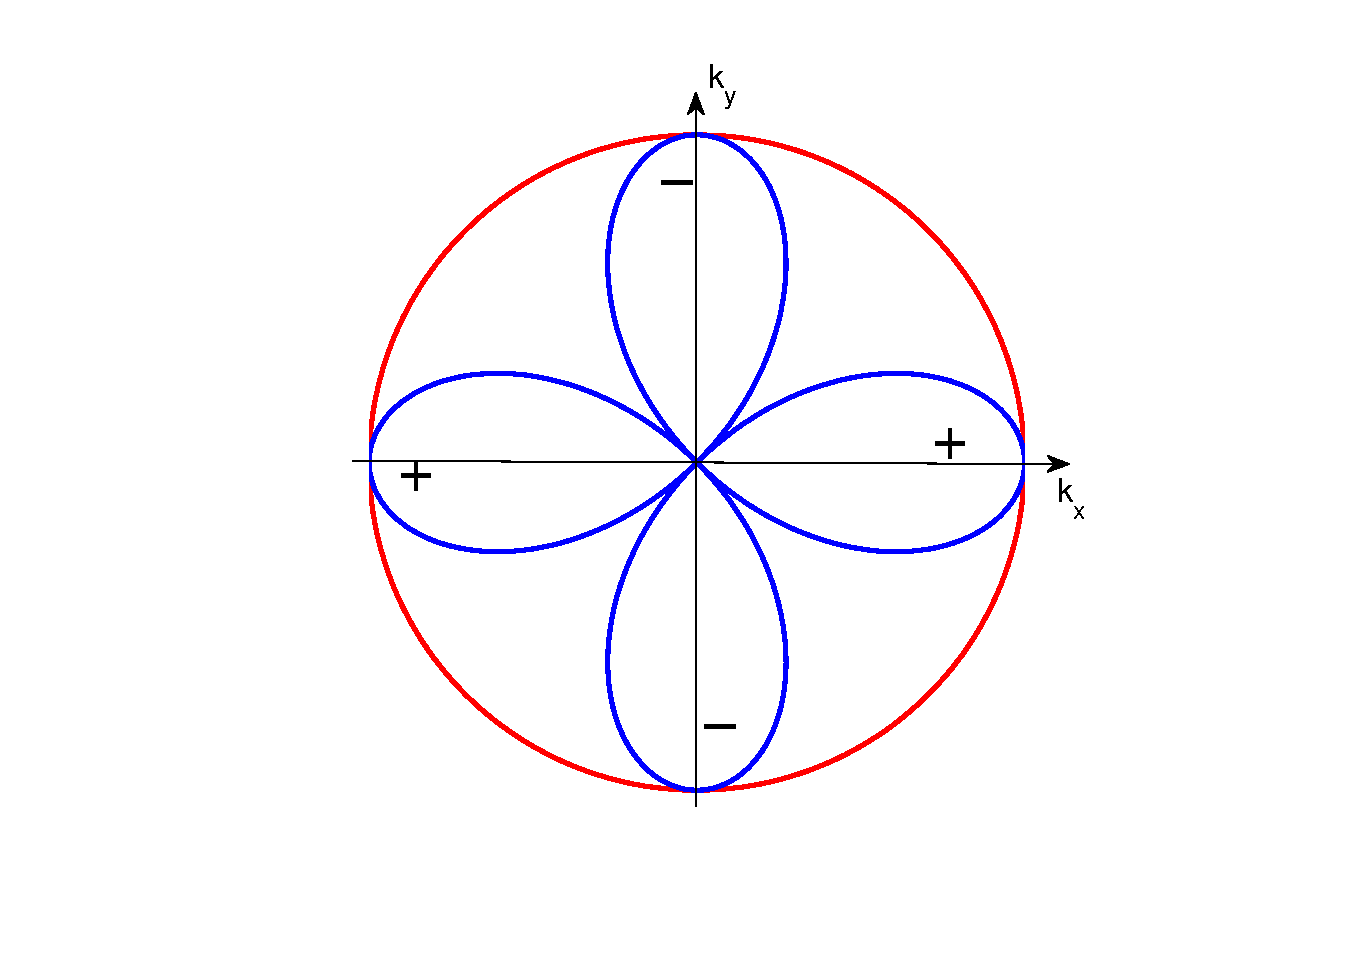
\includegraphics[width=10cm]{./Figures/2-1-1.eps}
\rule{35em}{0.5pt}
\caption[An Electron]{The shape of s-wave energy gap is a circle while that of d-wave energy gap is like a petal. Notice that the $d_{x^2-y^2}$ has two positive and negative leaves}
\label{Pair Potential Fig}
\end{figure}

\section{$D$-Wave Tunnelling Spectroscopy of Superconductors}
To approach the calculation of tunnelling spectroscopy of superconductors to fit the experimental results in our group, there are several steps to go in both theory and calculation. First of all, we need to establish the model for $s$-wave, the basis for the following calculations. Second, $s$-wave model serves the kernel so that it will guide us to the d-wave tunnelling spectroscopy results by conducting an integral over it. Finally, we obtain the conductances that can be compared to our BSCCO on BSC experiments. In addition, an algorithm for fitting the results is implemented.

We first introduce the formula for the conductance versus bias\citep{Reference6} before we discuss  the details of the d-wave tunnelling spectroscopy.  
\subsection{I-V Curve Function For N-S Boundary}
The reference\citep{Reference6} derives that the I-V curve for N-S Boundary could be written like
\begin{eqnarray}\label{BTK Conductance}
I_{NS}=2N(0)ev_F\mathcal{A}\int_{-\infty}^{\infty}[f_0(E-eV)-f_0(E)][1+A(E)-B(E)]dE
\end{eqnarray}
in which $f_0(E)$ is the fermi distribution and B(E) is the probability of normal reflection and A(E) is the probability of Andreev reflection, namely where the electron enters the superconductor as a cooper pair, while reflecting a hole.
\begin{eqnarray}
f_0(E) = \DF{1}{1+e^{(E-\mu)/kT}}
\end{eqnarray}
where $\mu$ is the chemical potential. 
By applying a differential operation on \eqref{BTK Conductance} we get that
\begin{eqnarray}\label{Conductance}
\sigma=\frac{\partial I}{\partial V}=\int_{-\infty}^{\infty}\sigma_T(E)\frac{\partial{f_0(E-eV)}}{\partial{V}}dE
\end{eqnarray}
Omitting the constant factor, the following term is what we are focusing on
\begin{eqnarray}\label{2D-Kernel}
&&\sigma_T(E) = \int d\Omega\sigma_S\cos\theta=\int d\Omega(1+A(E)-B(E))\cos\theta\nonumber\\
&&\sigma_S(E)=1+A(E)-B(E)
\end{eqnarray}
where $A(E)$ is the famous Andreev reflection and $B(E)$ is the ordinary reflection, and $\theta$ is the incident angle since we are only considering the current along the tunnelling axis\citep{Reference6}, the former of which reflects a hole and generate a Cooper pair in the superconductor side.

\subsection{Properties of Tunnelling Spectroscopy Kernel $\sigma_S$}
Let's first study the tunnelling spectroscopy kernel $\sigma_S$ shown in \eqref{2D-Kernel}.

The Bogoliubov equations can be analytically solved if we assume that the potential between the two materials is a $\delta$ function while energy gap is a step function \citep{Reference2}, demonstrated in Fig.\ref{fig:BTK Pair Potential}.
\begin{figure}[htbp]
\small
\centering
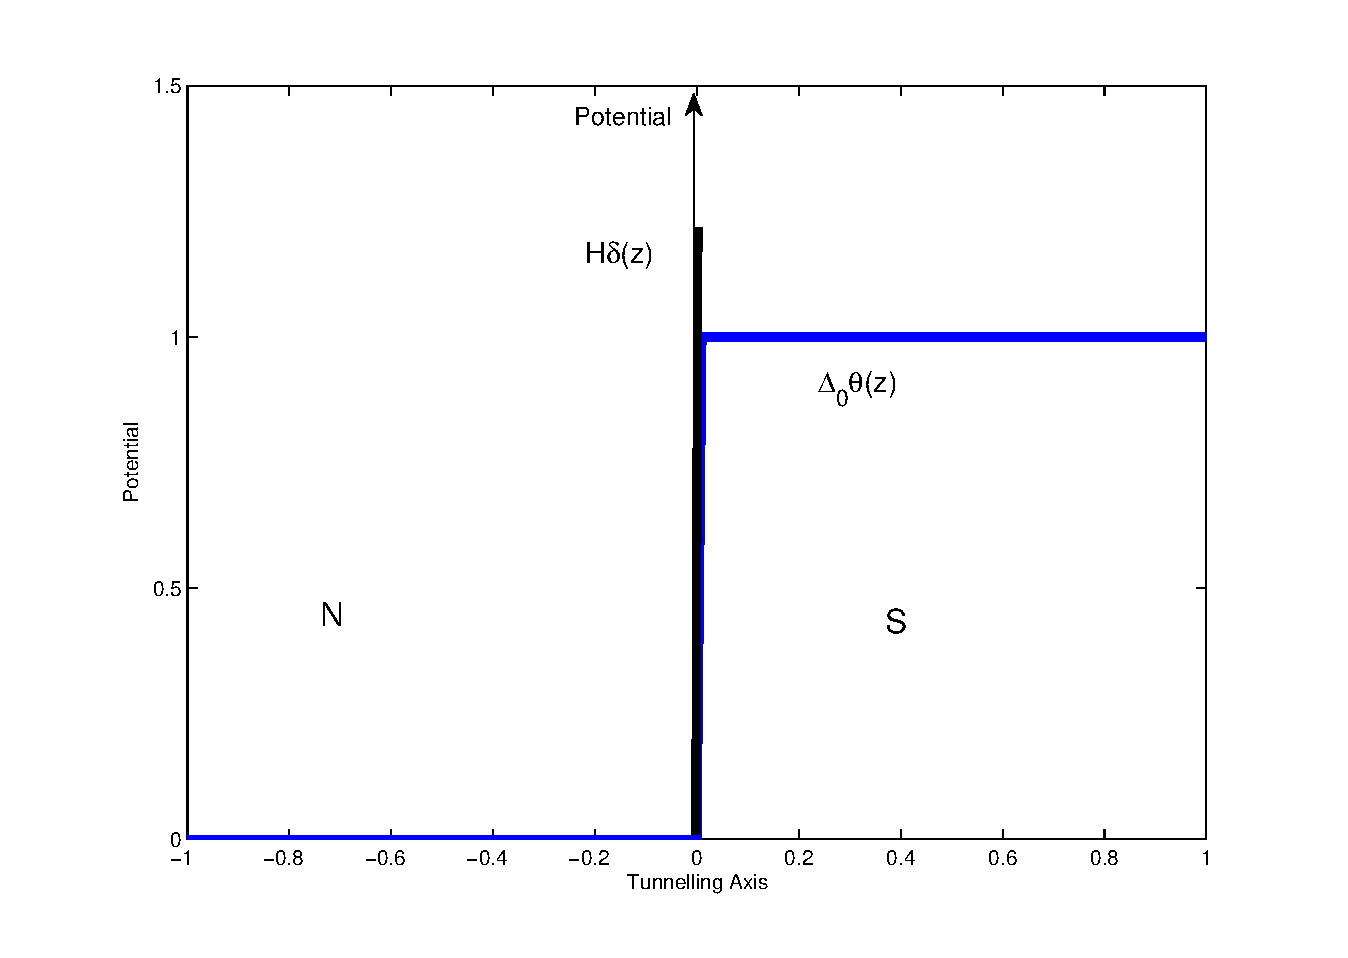
\includegraphics[width=10cm]{./Figures/2-2-1.eps}
\rule{35em}{0.5pt}
\caption[An Electron]{$\delta$ function of potential and step function of energy gap}
\label{fig:BTK Pair Potential}
\end{figure}
Also we define the effective pair potential $\Delta_+$ felt by the electron-like particles and effective pair potential $\Delta_-$ felt by the hole-like particles as following

\begin{eqnarray}\label{General Phase Pair}
\Delta_{\pm}=|\Delta_{\pm}|\exp(i\phi_{\pm})
\end{eqnarray}
From the analytical solutions of BdG equations, we obtain the kernel of \eqref{2D-Kernel}, which is written in \eqref{1DKernel}.
\begin{eqnarray}\label{1DKernel}
\sigma_R(E)=\frac{\sigma_S(E)}{\sigma_N}=\frac{1+\sigma_N\mid\Gamma_+\mid^2+(\sigma_N-1)\mid\Gamma_+\Gamma_-\mid^2}{\mid1+(\sigma_N-1)\Gamma_+\Gamma_-\exp(i\phi_--i\phi_+)\mid^2}
\end{eqnarray}
where the terms $\Gamma_{\pm}$,the normal conductance $\sigma_N$ and the effective barrier hight $Z$ are
\begin{eqnarray}
\Gamma_{\pm}=\frac{E-\sqrt{E^2-|\Delta_{\pm}|^2}}{|\Delta_{\pm}|},Z=\frac{Z_0}{\cos\theta},
\sigma_N=\frac{1}{1+Z^2}
\end{eqnarray} 
and we write the term $\sigma_S(E)$ for convenience.
\begin{eqnarray}\label{Tanaka Kernel}
\sigma_S(E)=\sigma_N\frac{1+\sigma_N\mid\Gamma_+\mid^2+(\sigma_N-1)\mid\Gamma_+\Gamma_-\mid^2}{\mid1+(\sigma_N-1)\Gamma_+\Gamma_-\exp(i\phi_--i\phi_+)\mid^2}
\end{eqnarray}
Fig.\ref{fig:Kernel Vary Z} indicates different shapes with different, $Z$, the barrier hight, where we assume that the phase difference $\phi_--\phi_+=0$.

\begin{figure}[htbp]
\small
\centering
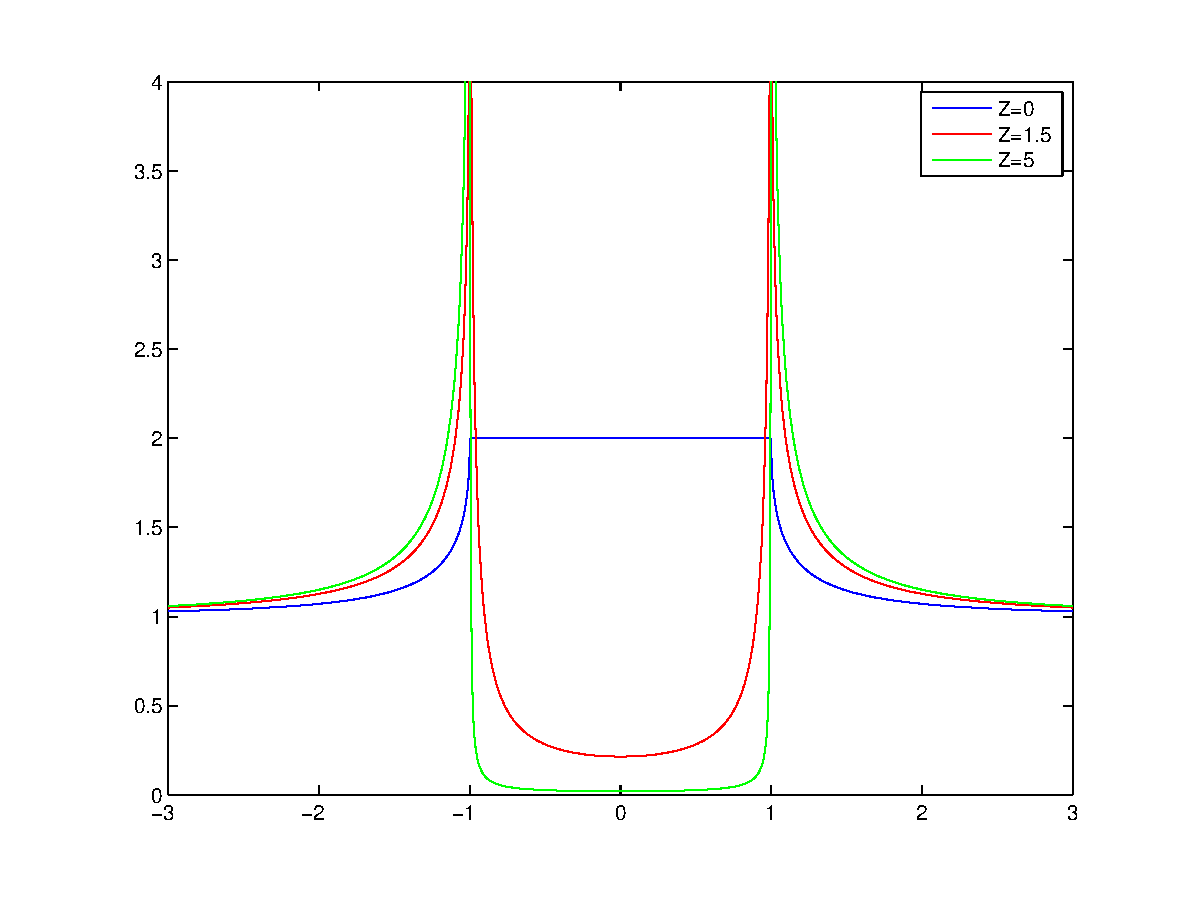
\includegraphics[width=10cm]{2-2-2.eps}
\caption{The picture indicates the different shapes of $\sigma_R(E)$ corresponding to the different barrier values. Here $\Delta_+=\Delta_-$}
\label{fig:Kernel Vary Z}
\end{figure}

The general function for the normalised tunnelling conductance $\sigma_T$ is 
\begin{eqnarray}\label{2D-Kernel-Integral}
\sigma_T(E)=\DF{\int d\Omega \sigma_S(E)\cos\theta}{\int d\Omega\sigma_N\cos\theta}
\end{eqnarray}
where we can see that the kernel $\sigma_S$ is implemented.
The integral operators in $d$-wave $ab$ tunnelling and in $c$-tunnelling is written as
\begin{eqnarray}\label{abc}
&&\int d\Omega^{(ab)}=\int_{-\pi/2}^{\pi/2} d\theta\nonumber\\
&&\int d\Omega^{(c)}=\int_{0}^{2\pi}d\varphi\int_{0}^{\pi/2} d\theta \sin\theta
\end{eqnarray}
$\varphi$ is the interface angle.

\subsection{$ab$-Tunnelling Spectroscopy}
The $d$-wave tunnelling spectroscopy has are two cases: $ab$ tunnelling whose tunnelling axis is normal to the $c$-axis of the crystal, and $c$ tunnelling whose tunnelling axis is parallel to the $c$-axis of the crystal, Fig.\ref{Pair Potential Fig}. We first of all discuss $ab$-tunnelling spectroscopy.

In fact, the averaged normal conductance in \eqref{2D-Kernel-Integral} can be derived directly.
\begin{eqnarray}
\overline{\sigma_N}=\int d\Omega^{(ab)} \sigma_N\cos\theta
\end{eqnarray}
so that
the averaged normal conductance is
\begin{eqnarray}
\overline{\sigma_N}=2-\frac{Z_0}{\sqrt{1+Z_0^2}}\ln\Big(\frac{\sqrt{1+Z_0^2}+1}{\sqrt{1+Z_0^2}-1}\Big)
\end{eqnarray}

Now we focus our discussion on the specific case of $d_{x^2+y^2}$, where in $ab$-tunnelling $\Delta_-,\Delta_+$ are written as
\begin{eqnarray}\label{ab pair potential}
\Delta_+=\Delta_0\cos2(\theta-\alpha)\nonumber\\
\\
\Delta_-=\Delta_0\cos2(\theta+\alpha)\nonumber
\end{eqnarray}
where $\theta$ represents incident angle, $\alpha$ the angle between the tunnelling axis and main axis of the pair potential, shown in Fig.\ref{fig:ab-tunnelling schematic}.
\begin{figure}[htbp]
\small
\centering
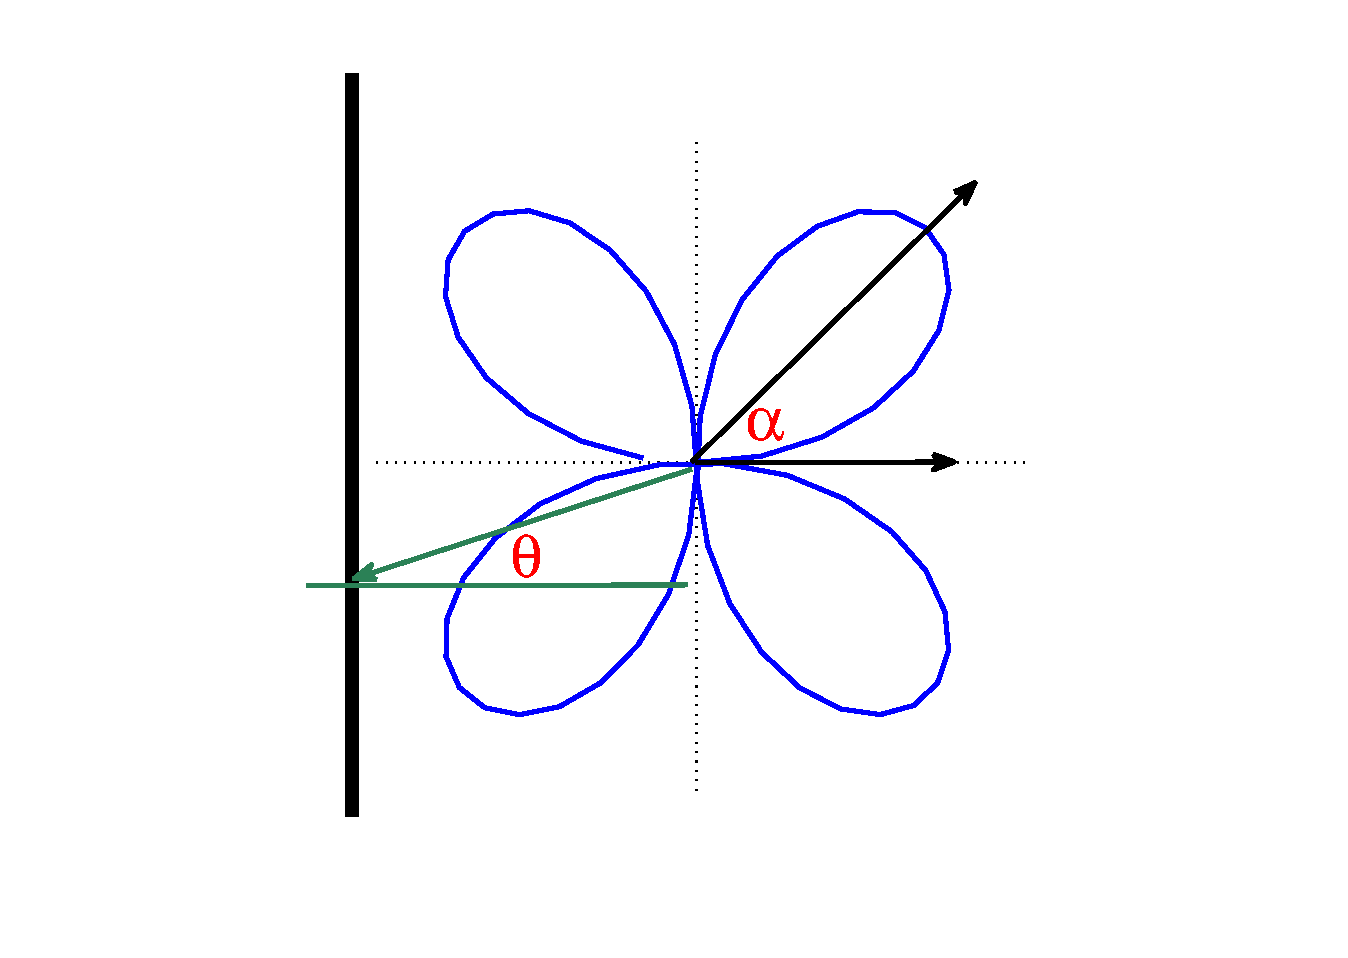
\includegraphics[width=10cm]{ab-tunnelling.eps}
\caption{Schematic illustration of the incident angle $\theta$ and the angle $\alpha$.}
\label{fig:ab-tunnelling schematic}
\end{figure}


Turning to Fig.\ref{fig:dc-alpha}, we see the shape of the conductance is sensitive to the incident angle and thus the phase difference 
\begin{eqnarray}\label{d wave phase difference}
e^{i\phi_--i\phi_+}=\frac{|\Delta_+|}{\Delta_+}\frac{\Delta_-}{|\Delta_-|}=\frac{|\cos2(\theta-\alpha)|}{\cos2(\theta-\alpha)}\frac{\cos2(\theta+\alpha)}{|\cos2(\theta+\alpha)|}\in\{-1,1\}
\end{eqnarray}

\begin{figure}[htbp]
\small
\centering
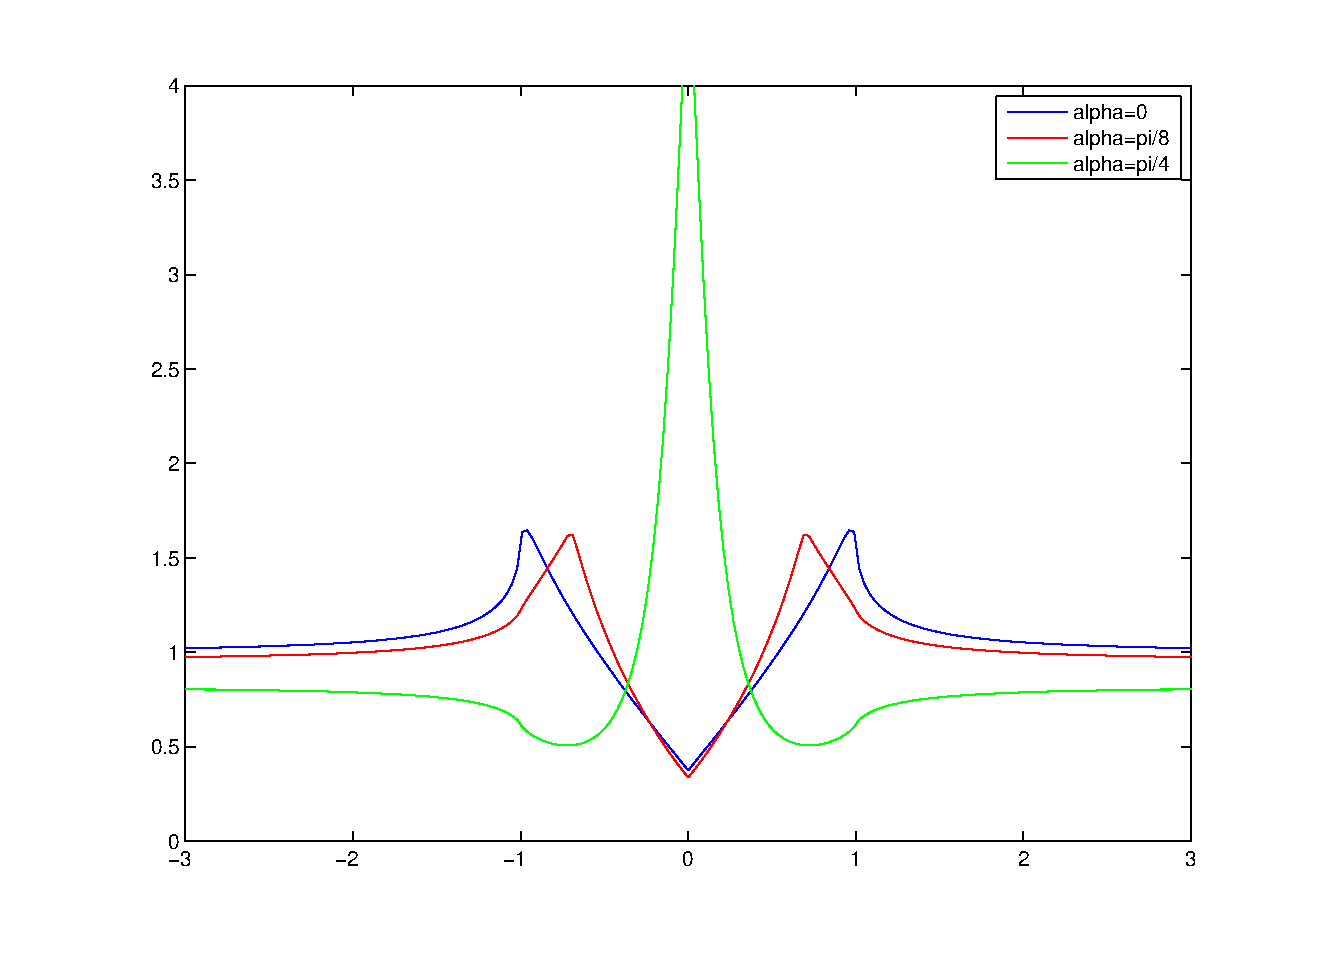
\includegraphics[width=10cm]{2-2-5.eps}
\caption{The figure indicates the correspondence of conductance and angle between incident normal and the petal axis.}
\label{fig:dc-alpha}
\end{figure}

Furthermore we limit the phase difference to zero. 

Fig.\ref{fig:dc-gap} shows the property of the $ab$ tunnelling spectroscopy respect to different pair potentials, which indicates that one pair potential corresponds to one peak in the figure, while if pair potential is zero, the tunnelling conductance is a constant, $1$.
\begin{figure}[htbp]
\small
\centering
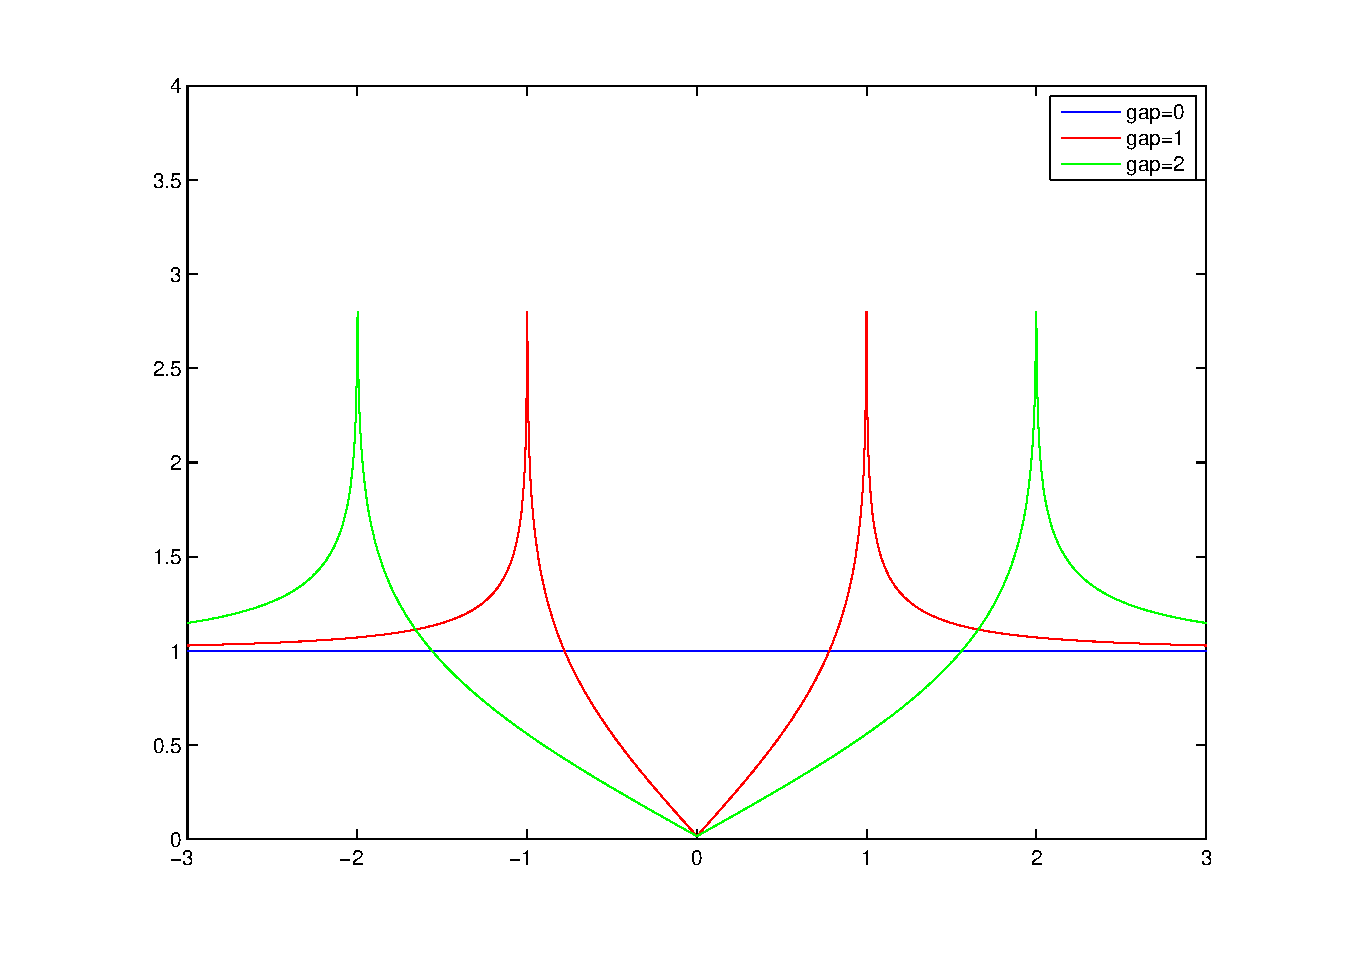
\includegraphics[width=10cm]{2-2-4.eps}
\caption{The figure demonstrates the total tunnelling conductance with different
energy gaps. When energy gap amplitude is zero, the peaks vanish, meaning
that the material turns into normal metal. Here we choose $Z=5$}
\label{fig:dc-gap}
\end{figure}

\subsection{Differential Conductance with Different Temperatures and Fixed Energy Gap Amplitude}
In general, the properties of differential conductance is determined by the derivative of the fermi function and tunnelling conductance kernel, according to \eqref{Conductance} and \eqref{1DKernel}.
As an illustration,Fig.\ref{fig:fermi-dc} shows differential conductance at Temperature 1K, where the top figure is the differential conductance, the bottom figure is the tunnelling conductance, and the others are the derivatives of fermi function at different biases. We see that the peak of the derivatives are close to $\delta$ functions, which makes the differential conductance look similar to the tunnelling conductance after the integration.
\begin{figure}[htbp]
\small
\centering
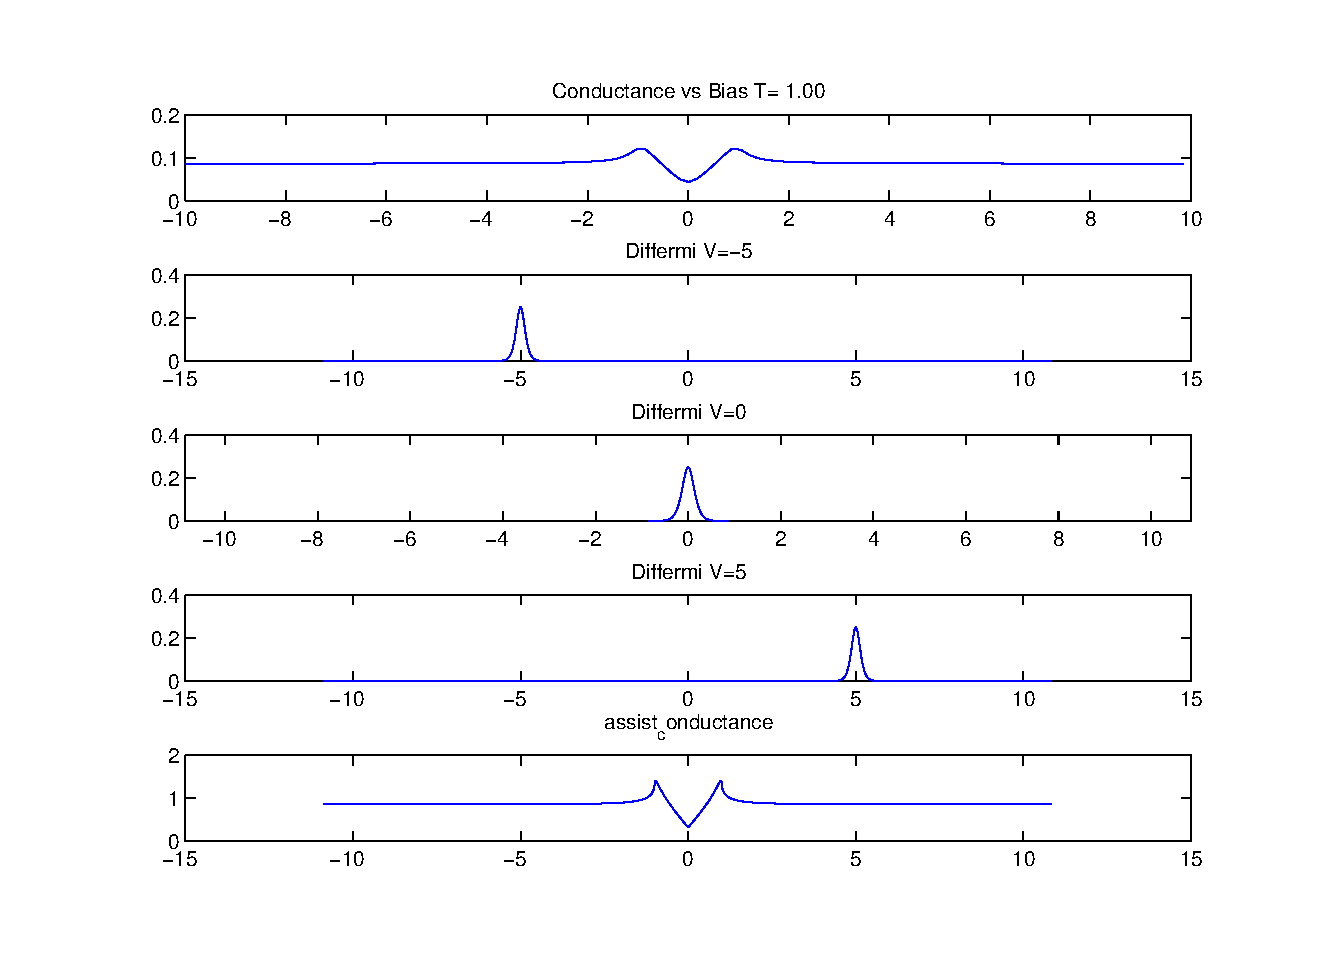
\includegraphics[width=12cm]{2-2-6.eps}
\caption{Differential conductance with T=1K, accompanied by plots of three derivatives of the fermi distributions at varied biases and  a tunnelling conductance graph in the bottom.}
\label{fig:fermi-dc}
\end{figure}

Let's discuss a way to make the picture more clear in Fig.\ref{fig:3D-dc}, demonstrating the relation between the tunnelling conductance with temperature with a FIXED pair potential. We could observe that the dip in middle generally vanish as the temperature increases.
\begin{figure}[htbp]
\small
\centering
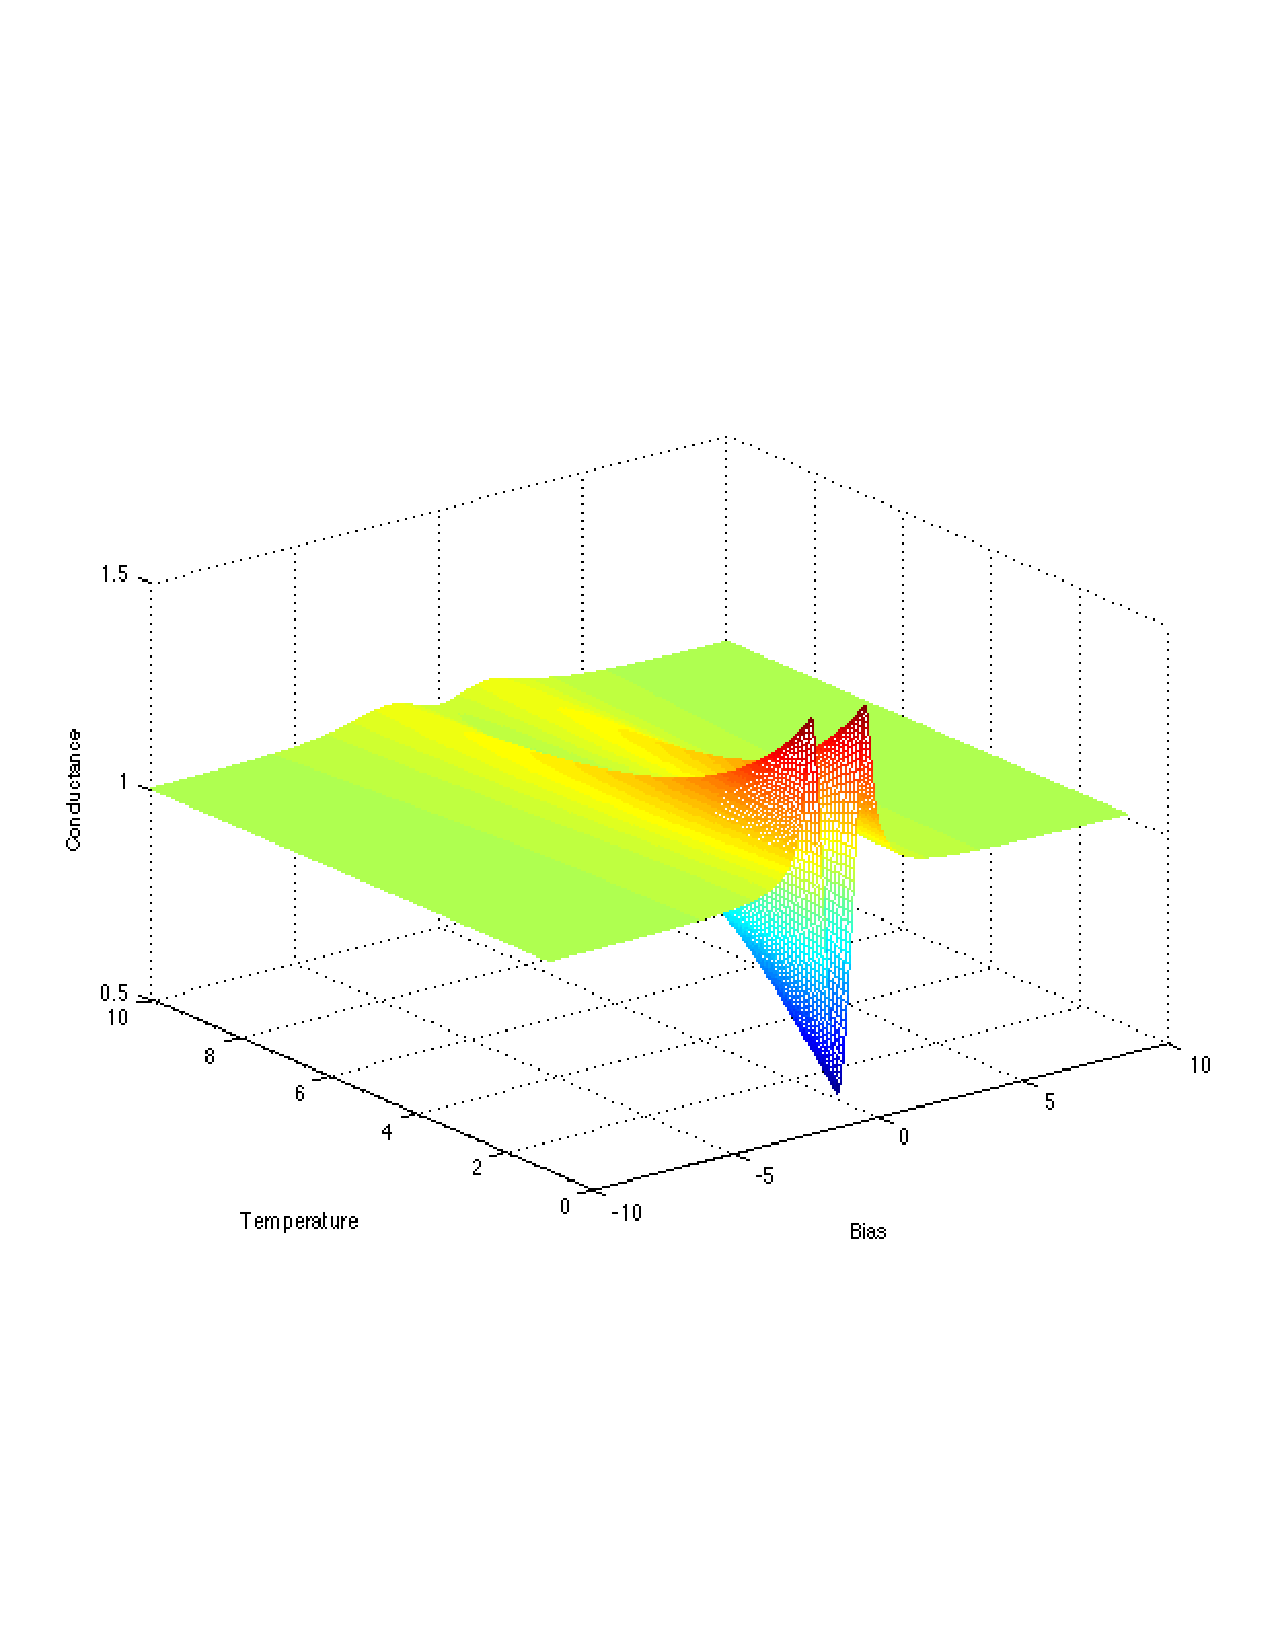
\includegraphics[width=12cm]{2-2-8.pdf}
\caption{This figure indicates the relation between temperature, bias and the conductance.The different colours indicate the temperature.}
\label{fig:3D-dc}
\end{figure}

\subsection{Differential Conductance with Different Pair Potential Amplitudes with Fixed Temperature}
Though we should be clearly warned that the energy gap is dependent on the temperature, we still do a study for the relation between differential conductance with energy gap amplitudes.

Generally, the shapes of tunnelling conductance are similar except when the energy gap amplitude is zero, which will make the tunnelling conductance constant, already indicated in Fig.\ref{fig:dc-gap}.

Therefore, we simply provide an illustration figure. We could notice that with the increase energy gap amplitude, the centre dip becomes deeper, Fig.\ref{fig:3D-dc-gap}.
\begin{figure}[htbp]
\small
\centering
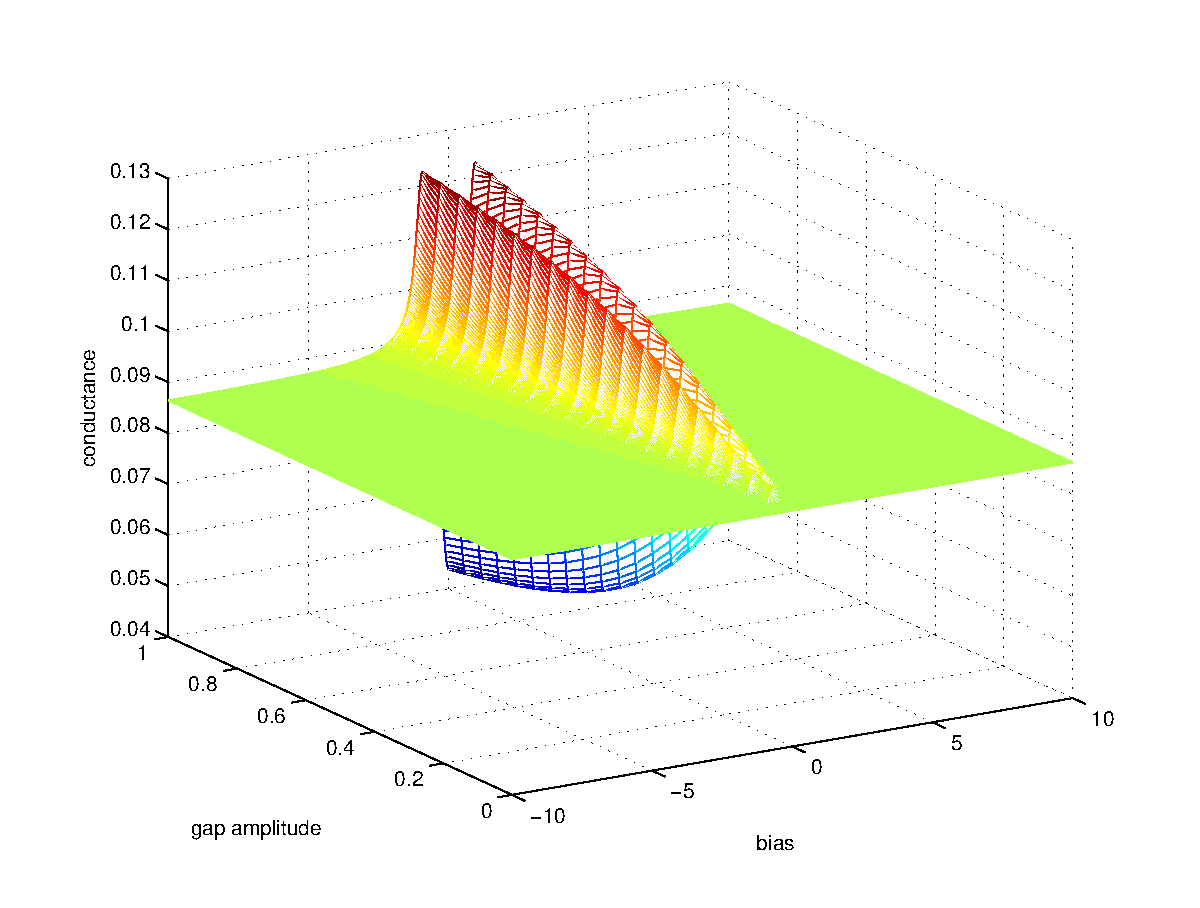
\includegraphics[width=12cm]{2-2-9.eps}
\caption{This figure indicates the relation between energy gap amplitude, bias and the conductance.}
\label{fig:3D-dc-gap}
\end{figure}


Now we briefly introduce the calculation methods. It should be noted that we are trying to calculate a second order integral, which may lead to a large calculation time, as that we might have to calculate $1000\times1000$ volume. I developed a simple method based on the essential features of function $\sigma_S$ and differential fermi distribution function $\frac{\partial{f_0(E-eV)}}{\partial{V}}$ in the integrations\eqref{Conductance} and \eqref{2D-Kernel-Integral}.

First of all, the function $\sigma_T(E)$ is assumed to be  CONSTANT when parameter E's absolute value is to some extent larger than amplitude of the energy gap, Fig.\ref{fig:dc-gap}.

Second, we note that differential fermi distribution function is actually of Delta function type, which means the value could be assumed zero when its parameter $E-\mu-eV$ is "much" larger than $kT$. Also, all the derivatives of the fermi distribution function shares the exact shape, shown in Fig.\ref{fig:fermi-dc}; their only difference is that the peaks are in different positions corresponding to the value of bias.

With the above knowledge, we calculate the the tunnelling spectroscopy point values according to a chosen step length ONLY ONCE and store the data. When parameter $E$ is "large", we use constant for the point. We define this as calculation (1).
Also, we calculate the point values of the derivative of the fermi distribution function at bias zero according to the step length used in the calculation (1). When parameter $E-\mu-eV$ is "large", we make the point value as zero. When We define this as calculation (2).
Since calculation (1) and calculation (2) share the same step length, if we need to calculate the differential conductance at a certain bias, we translate the point values of the derivative to that bias and do the integration limited to the non-zero points of the derivative.
To avoid losing information, the choice of the step length is significant. We choose step length according to the smaller value of peak width between the differential fermi distribution function and tunnelling conductance.
The method remarkably improves the performance of the calculation yet loses very little accuracy. The weakness of this method is that the computation is slow when energy gap amplitude is small while the temperature is high, which, however, is easily to be removed by adding some plotting and integrating step boundaries.

\subsection{$c$-Tunnelling Spectroscopy and Fitting the Experimental Data}
As our experiments are conducted with the materials along $c$-axis of d-wave pair potential, we now focus on this case. The schematic illustration is shown in Fig.\ref{fig:c-tunnelling schematic}.
\begin{figure}[htbp]
\small
\centering
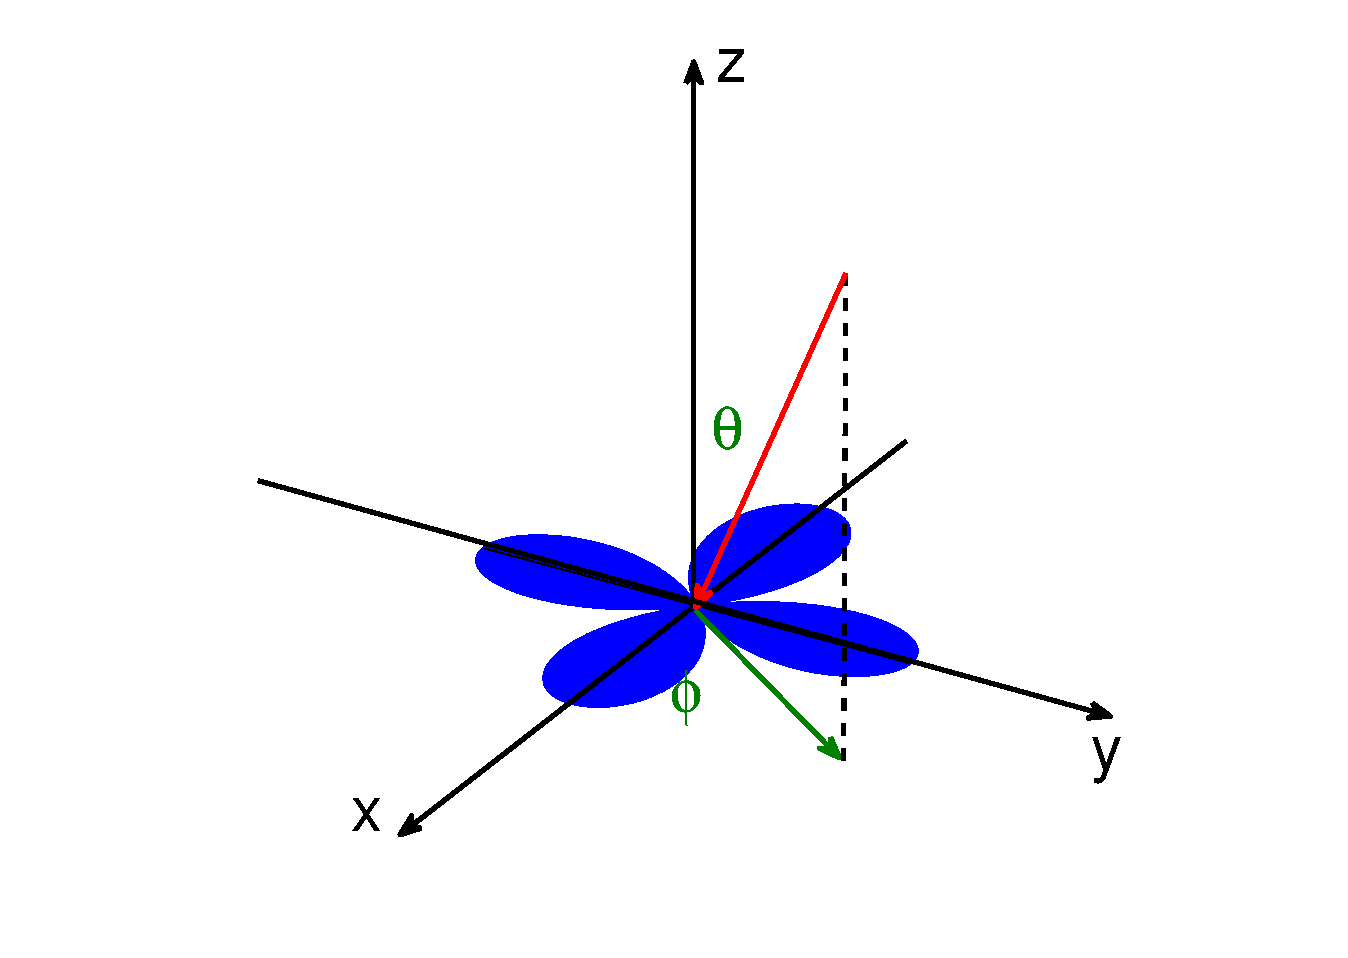
\includegraphics[width=12cm]{./Figures/c-tunnelling.eps}
\caption{The schematic illustration of $c$-tunnelling, where the incident angle $\theta$ and the interface angle $\varphi$ are indicated. In the figure, $x-y$ plane is the tunnelling interface.}
\label{fig:c-tunnelling schematic}
\end{figure}
The pair potential in $c$-tunnelling is written as
\begin{eqnarray}
\Delta(\varphi)=\Delta_0\cos2\varphi
\end{eqnarray}
The averaged N-I-N junction conductance over the half-sphere of $k$ space could be calculated directly.
According to the formula in the following, that calculates the averaged normal conductance,
\begin{eqnarray}
\overline{\sigma_N}=\int_0^{2\pi}d\phi \int_{0}^{\frac{\pi}{2}} d\theta \cos\theta\sin\theta \sigma_N
\end{eqnarray}
where we assume that 
\begin{eqnarray}
\sigma_N=\DF{1}{1+(\DF{Z_0}{\cos\theta})^2}
\end{eqnarray}
We could simply calculate the integral for averaged normal conductance,
\begin{eqnarray}\label{average-normal}
\overline{\sigma_N}=\pi \Big[1-Z_0^2\ln\Big(1+\DF{1}{Z_0^2}\Big)\Big]
\end{eqnarray}
Knowing the formula \eqref{average-normal}, we could step over the numerical integral of normal conductance. Ideally, it also can be used to calculate the barrier hight.
 
Typically the $c$-tunnelling spectroscopy is similar to that of $ab$-tunneling, when alpha = 0, since the incident angle averages over the d-wave gap in a similar manner. 

We conducted an experiment about the tunnelling spectroscopy with the layers of the material Bismuth strontium calcium copper oxide having the generalised chemical formula $Bi_2Sr_2Ca_{n-1}Cu_nO_{2n+4+x}$ (BSCCO) and Calcium doped $Bi_2Se_3$(BSC), the former of which serves as a cuprate superconductor \citep{BSCCO} and the latter of which serves as a topological insulator\citep{Semiconductor}. We use $d$-wave $c$-tunnelling model to fit the experimental data.
Fig.\ref{fig:fitting} shows the fitting results for our BSCCO on BSC experimental results by manually inputting the parameters.
 \begin{figure}[htbp]
\small
\centering
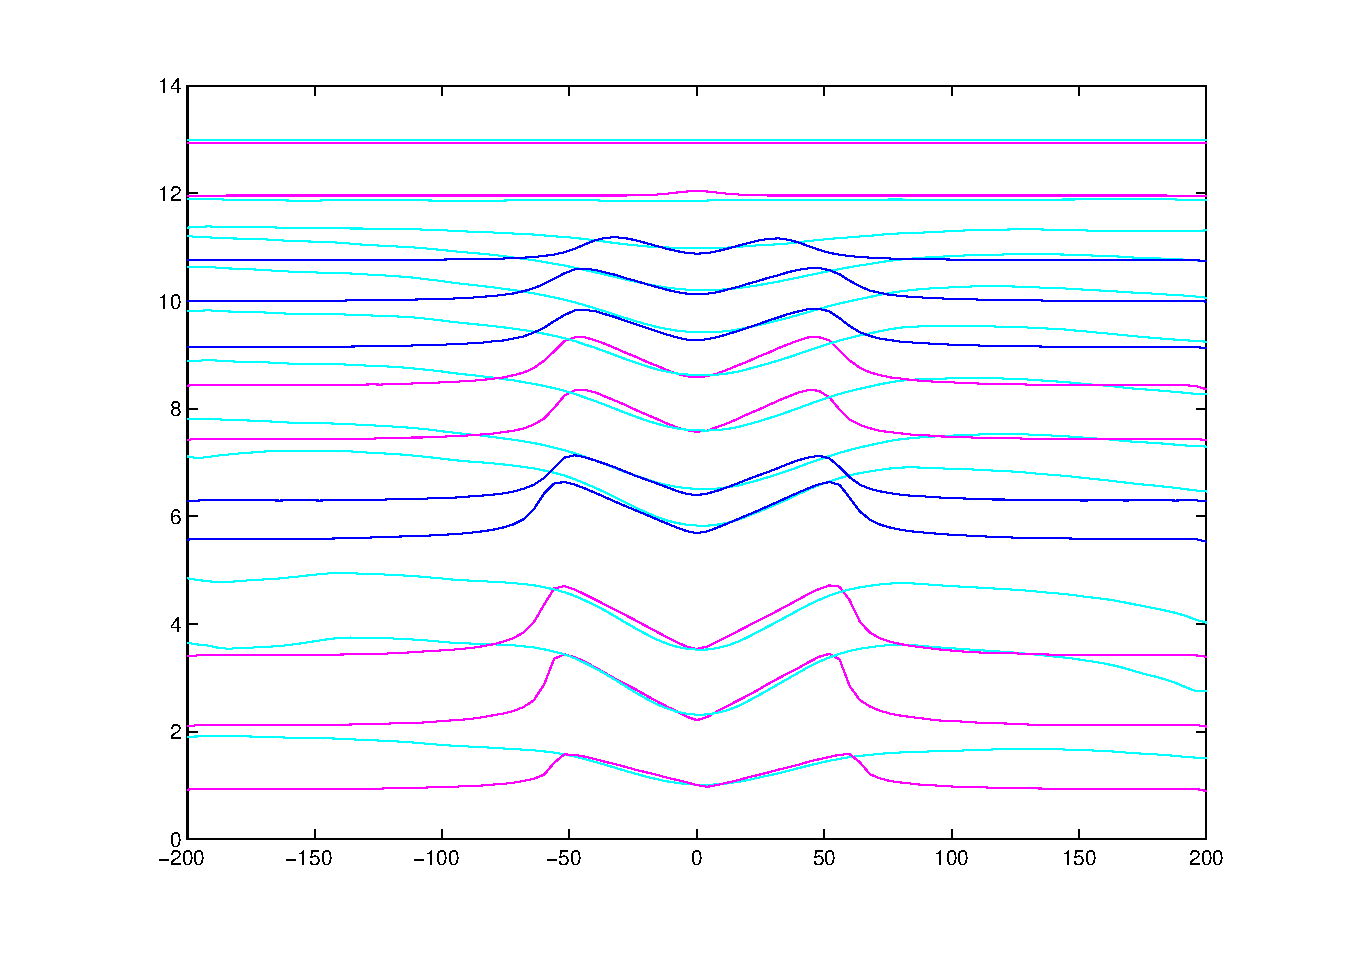
\includegraphics[width=12cm]{./Figures/Fitting.eps}
\caption{Conductances normalised by 70K with Temperature, where the deep colour represents calculation. Each bundle represents, from bottom to top, sequentially,  $10K$,$13K$,$15K$,$30K$,$35K$,$40K$,$45K$,$50K$,$55K$,$65K$,$70K$.}
\label{fig:fitting}
\end{figure}

And chosen energy gaps versus temperature for fitting the experimental data are shown below, Fig.\ref{fig:fit pair potential}.
 \begin{figure}[htbp]
\small
\centering
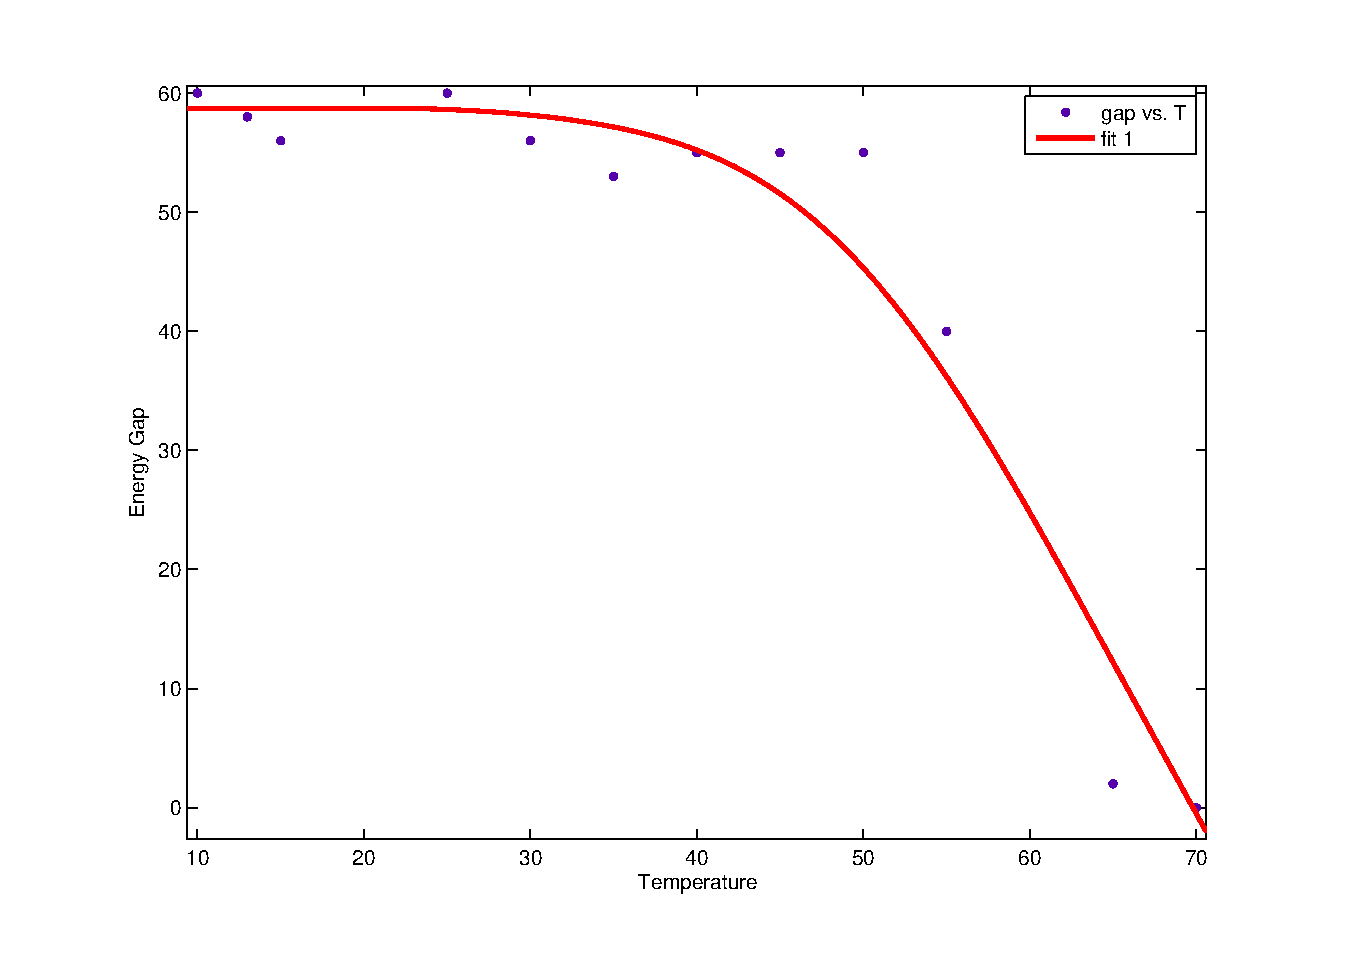
\includegraphics[width=8cm]{gap.eps}
\caption{Energy Gaps with Temperature}
\label{fig:fit pair potential}
\end{figure}


The fitting results are not satisfactory. Only in the dip part the fitting results agree to some extent with the experimental results. But at the both sides they are quite far away. The reason for this disagreement is that the model we use is for low temperature case and is based on the assumption that the density of states is a constant at (2.12) and the properties of our model is determined by the integration kernel of (2.19), which also has peaks at the point $E=\Delta_0$. The experiment results, however, do not have the corresponding peaks, leading to the fact that the fitting results only match a small part of the experimental results in the centre.

To try to eliminate of the disagreement from the computational part, we implemented the genetic algorithm for fitting the data\citep{GA}.

Genetic algorithm(GA) is an optimisation heuristic inspired by the natural selection process in biological systems. Very similar to the selection process, GA maintains a population of candidates and process mechanisms of encoding, selection, crossover, mutation and culling in the population\citep{GA}. 

In the calculation, we select a population of 50 for the desired parameters randomly generated within the set range and calculate the fitness value, such as standard error and then sort the population according to the fitness value increasingly. Second, we choose the first 25 of the population according to the sorted list as parents while we select another 25 samples of the population as mutants randomly multiplied by some restricted random numbers. 25 selected parents will generate 25 offsprings by crossover. Then we mix the original population, the generated offspring as well as the 25 mutants together to compose a country of 100 samples. Third, we do sorting again with the population the eliminate the last 50 samples of the population. We will repeat the above three steps until the termination requirement is satisfied. 

The above statement is the ideal approach to fit the experimental data, while unfortunately the results come out not satisfactory.










































 % Background Theory 

% Chapter 1
%\newcommand {\DF}[2]{{\displaystyle\frac{#1}{#2}}}
\chapter{Tunnelling Spectroscopy with Proximity Effect} % Write in your own chapter title
\label{Chapter3}
\lhead{Chapter 3. \emph{Tunnelling Spectroscopy with Proximity Effect}} % Write in your own chapter title to set the page header

It is interesting to propose a theory calculating the $d$-wave conductance accounting for the proximity effect as required by our novel experiments. In this chapter, we limit our discussion to $s$-wave and $d_{x^2-y^2}$ cases.

Identical to the steps mentioned in the last chapter. We first solve the Bogoliubov equations and study the properties of the the tunnelling conductance kernel, $\sigma_S$ in (2.25). Then the knowledge of the conductance kernel, $\sigma_S$ will guide us to the desired $d$-wave proximity conductance.
Currently this work is in progress.
\section{Bogoliubov Equations}
As a matter of fact, the tunnelling conductance discussed in the previous chapter is based on a specific case which is shown in Fig.2.2. The potential is assumed as a $\delta$ function and the pair potential is assumed as a step function, so that Bogoliubov  equations(3.1) have an analytic solution. In contrast, such analytic solution no longer exists when dealing with more complicated case accounting for proximity effect where the gap is not simply a step function.
\subsection{Simplification for the Bogoliubov Equations}
The general Bogoliubov equations are 
\begin{eqnarray}\label{eq:GeneralBDG}
i\hbar\frac{\partial f}{\partial t} = \Big(-\frac{\hbar^2}{2m}\frac{\partial^2}{\partial {z^2}}-\mu(z)+V(z)\Big)f(z,t)+\Delta(z)g(z,t)\nonumber\\
\\
i\hbar\frac{\partial g}{\partial t} = \Big(-\frac{\hbar^2}{2m}\frac{\partial^2}{\partial {z^2}}-\mu(z)+V(z)\Big)g(z,t)+\Delta(z)f(z,t)\nonumber
\end{eqnarray}
Here we set $z$ as our tunnelling axis.
\eqref{eq:GeneralBDG} has the solution form 
\begin{eqnarray}
\varphi(z,t)=
\left(\begin{array}{c}
f(z,t)\\
g(z,t)
\end{array}\right)
\end{eqnarray}
where $\mu(z),\Delta(z),V(z)$ are chemical potential, energy gap, and the ordinary potential which is related to the barrier height, in which we are interested in the latter two.
By introducing a solution of the form in terms of the wave vector
\begin{eqnarray}\label{eq:wavefront}
f=u(z)e^{i\mathbf{k}_F\cdot\mathbf{z}-\frac{iEt}{\hbar}}\nonumber\\
\\
g=v(z)e^{i\mathbf{k}_F\cdot\mathbf{z}-\frac{iEt}{\hbar}}\nonumber\
\end{eqnarray}
$\mathbf{z}$ is the tunnelling axis vector. And $\mathbf{k_F}$ represents the fermi vector, whose amplitude $k_F$ is a CONSTANT for $d_{x^2-y^2}$-wave case and $s$-wave case. And we relate it to the coherence length, another CONSTANT.
\begin{eqnarray}\label{fermi vector}
\xi_0=\hbar v_F/(\pi\Delta_0)=\hbar^2k_F/(\pi m \Delta_0)
\end{eqnarray}
The term $\Delta_0$ is used in the expression \eqref{energy gap k and z} for $s$-wave and $d_{x^2-y^2}$ cases
\begin{eqnarray}\label{energy gap k and z}
&&\Delta(\mathbf{k},z)=\Delta_0\Delta(z)\Delta(\mathbf{k})\nonumber\\
&&\left.\Delta(z)\right|_{z=+\infty}=1,\left.\Delta(z)\right|_{z=-\infty}=0
\end{eqnarray}
We also define the following function for convenience
\begin{eqnarray}\label{delta infty}
\Delta_{\infty}=\Delta(\mathbf{k},+\infty)=\Delta(\mathbf{k})
\end{eqnarray}
The Bogoliubov equations could be written in this way neglecting higher order terms\citep{Reference4}.
\begin{eqnarray}\label{eq:BdG}
&&\DF{\partial u}{\partial z}=i(\pi \xi_0\Delta_0\cdot(\widehat{\mathbf{k}}\cdot\widehat{\mathbf{z}}))^{-1}[Eu-\Delta(z)v]\nonumber\\
&&\DF{\partial v}{\partial z}=-i(\pi \xi_0\Delta_0\cdot(\widehat{\mathbf{k}}\cdot\widehat{\mathbf{z}}))^{-1}[Ev-\Delta(z)u]\nonumber\\
&&\widehat{\mathbf{k}}=\frac{\mathbf{k}}{|\mathbf{k}|},\widehat{\mathbf{z}}=\frac{\mathbf{z}}{|\mathbf{z}|}
\end{eqnarray}
which are the equations we are interested in, $\xi_0$ is the coherence length. Also we have the accompanied boundary conditions taking into account the potential $V(z)=Z_0(\pi\xi_0\Delta_0)\delta(z)$
\begin{eqnarray}\label{eq:OridinaryBoundary}
&&\left.\varphi\right|_{z=0^+}=\left.\varphi\right|_{z=0^-}\nonumber\\
\\
&&\left.\frac{\partial \varphi}{\partial z}\right|_{z=0^+}-\left.\frac{\partial \varphi}{\partial z}\right|_{z=0^-}=\left.2k_FZ_0\varphi\right|_{z=0^+}\nonumber
\end{eqnarray}

As indicated in the reference\citep{Reference4}, the Bogliubov equations are solved region by region, which finally lead us to the tunnelling conductance kernel. 
\begin{eqnarray}\label{sub-kernel}
\sigma_S=1+A-B
\end{eqnarray}
The andreev reflection $A$ and ordinary reflection $B$ in \eqref{sub-kernel} could be directly calculated from the solutions from the Bogliubov equations.

\subsection{Solving the Bogoliubov Equations}
We divide the tunnelling axis into four regions, named 'super','reduced','induced','normal', respectively, which is shown in Fig.3.1, where we already choose parabolic shape for the pair potential.
\begin{figure}[htbp]
\small
	\centering
		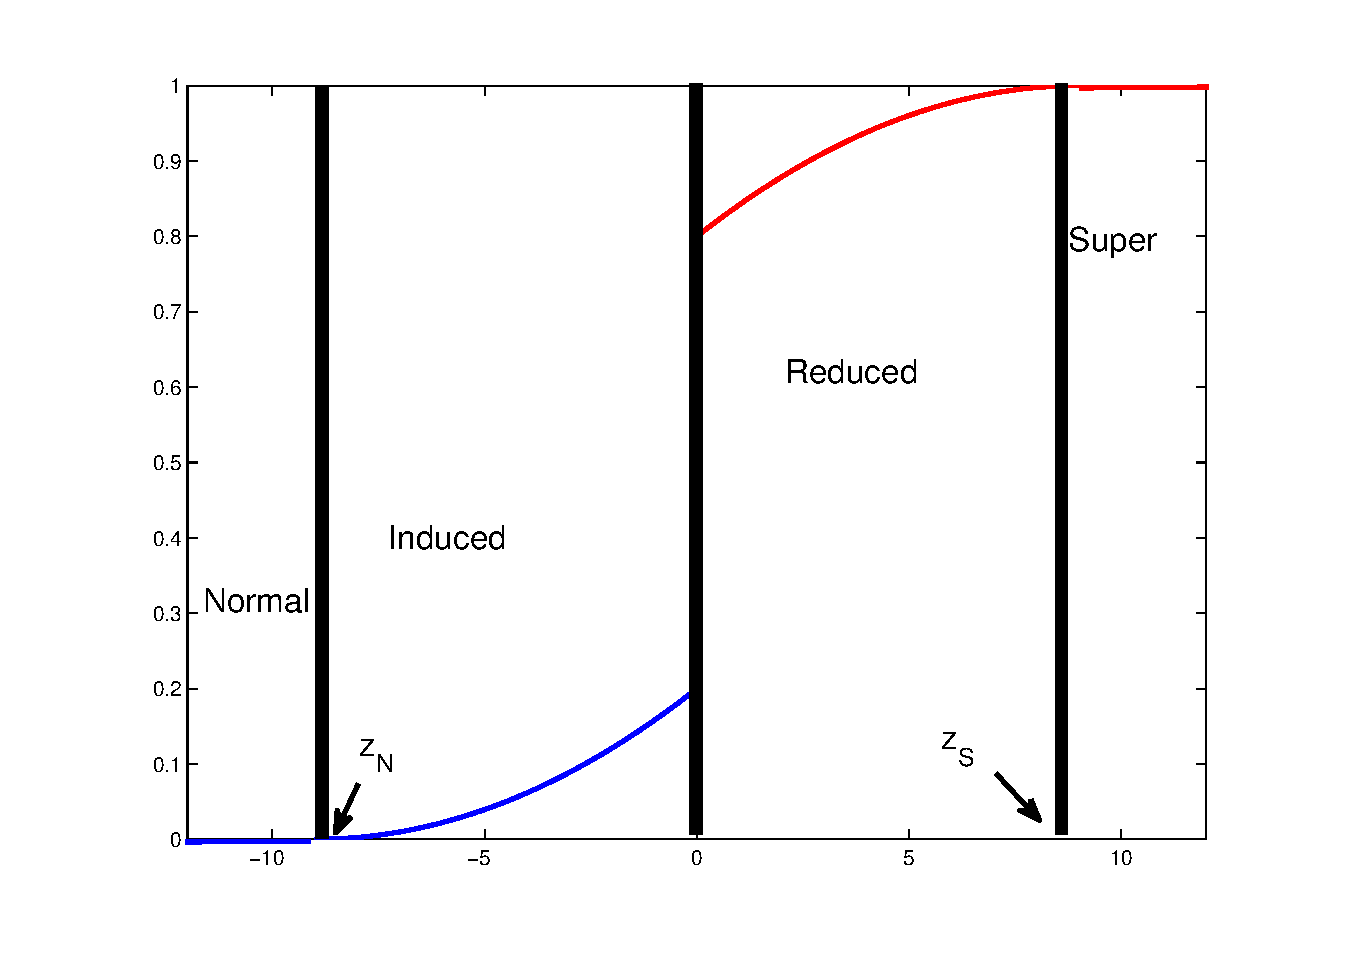
\includegraphics[width=10cm]{./Figures/3-2-1.eps}
		\rule{35em}{0.5pt}
	\caption[An Electron]{Parabolic shapes of reduced and induced pair potential. The tunnelling axis is divided into four regions.}
	\label{fig:EnergyGap}
\end{figure}
Now we solve the Bogoliubov equations region by region.

$\mathbf{\bullet \ 'Super'  \  Region}$

In the 'super' region, we already know the solution in \eqref{eq:superform}-\eqref{eq:superpara2}.
\begin{eqnarray}\label{eq:superform}
&&\varphi_1=
\left(
\begin{array}{c}
 u_0\\
 v_0
 \end{array}\right)e^{i(\mathbf{k}_F+\mathbf{k}'_S)\cdot\mathbf{z}}\nonumber\\
&&\\
&&\varphi_2=
\left(
\begin{array}{c}
 v_0\\
 u_0
 \end{array}\right)e^{-i(\mathbf{k}_F-\mathbf{k}'_S)\cdot\mathbf{z}}\nonumber
\end{eqnarray}
where parameters are already known,
\begin{eqnarray}\label{eq:superpara1}
u_0^2=1-v_0^2=\frac{1}{2}\Big(1+\frac{(E^2-\Delta_{\infty}^2)^{\frac{1}{2}}}{E}\Big)
\end{eqnarray}
where $\Delta_{\infty}$ is defined in \eqref{delta infty} and 
\begin{eqnarray}\label{eq:superpara2}
k_S'=k_S/(\widehat{\mathbf{k}}\cdot\widehat{\mathbf{z}})=(E^2-\Delta_{\infty}^2)^{1/2}(\pi \xi_0 \Delta_0(\widehat{\mathbf{k}}\cdot\widehat{\mathbf{z}}))^{-1}
\end{eqnarray}
The solution of this region serves as the generator of boundary conditions \eqref{reduceboundary} for the solution of the next region,'reduced' by applying the continuity of the wave functions $\varphi$ and the derivative of the wave functions $\partial\varphi/\partial z$. 

$\mathbf{\bullet \ Reduced \ Region}$
The solution of reduced region is assumed to have the form \eqref{reducedform}.
\begin{eqnarray}\label{reducedform}
\varphi_j=
\left(
\begin{array}{c}
 u_{aj}\\
 v_{aj}
 \end{array}\right)e^{i\mathbf{k}_F\cdot\mathbf{z}}+
 \left(
\begin{array}{c}
 v_{bj}\\
 u_{bj}
 \end{array}\right)e^{-i \mathbf{k}_F\cdot\mathbf{z}},j=1,2
\end{eqnarray}
Realising that $\mathbf{k}'_S\cdot\mathbf{z}=k_S/\cos\theta\widehat{\mathbf{k}}\cdot\widehat{\mathbf{z}}=k_Sz$ according to \eqref{eq:superpara2}, the boundary condition for the reduced region is
\begin{eqnarray}\label{reduceboundary}
&&u_{a1}(z_S)=u_{b2}(z_S)=u_0 e^{ik_Sz_S}\nonumber\\
&&v_{a1}(z_S)=v_{b2}(z_S)=v_0 e^{ik_Sz_S}\nonumber\\
&&\\
&&u_{b1}(z_S)=u_{a2}(z_S)=0\nonumber\\
&&u_{b1}(z_S)=u_{a2}(z_S)=0\nonumber
\end{eqnarray}
The term $z_S$ and $z_N$ are shown in Fig.\ref{fig:EnergyGap} and indicate the boundary of the reduced region with the super region and the normal region with the induced region respectively.
After obtaining the numerical solutions for \eqref{reducedform}, we select the values of only one point, which is at $z=0$
\begin{eqnarray}
&&u_{a1}(0)=u_{b2}(0)=u_{a1}^+\nonumber\\
\\
&&v_{a1}(0)=v_{b2}(0)=v_{a1}^+\nonumber
\end{eqnarray}
Before we move to the induced region, we make use of the original boundary condition at $z=0$, setting $V(z)=Z_0(\pi\xi_0\Delta_0)\delta(z)$.  In the boundary conditions \eqref{0condition}, the symbols $+,-$ represent $z=0^+,z=0^-$, respectively.
\begin{eqnarray}\label{0condition}
&&\left.\varphi\right|_{z=0^+}=\left.\varphi\right|_{z=0^-}\nonumber\\
\\
&&\left.\frac{\partial \varphi}{\partial z}\right|_{z=0^+}-\left.\frac{\partial \varphi}{\partial z}\right|_{z=0^-}=\left.2k_FZ_0\varphi\right|_{z=0^+}\nonumber
\end{eqnarray}
We neglect terms $u_{b1}(z), u_{a2}(z), v_{b1}(z), v_{a2}(z)$as they are zero because they have $0$ initial values in \eqref{reduceboundary}. 

$\mathbf{\bullet \ Induced \ Region}$
In light of the boundary conditions \eqref{0condition}, we write the solution of the induced region in the form of
\begin{eqnarray}\label{induced form}
&&\varphi_1=
(1+iZ)\left(
\begin{array}{c}
 u_{a0}\\
 v_{a0}
 \end{array}\right)e^{i\mathbf{k}_F\cdot\mathbf{z}}-iZ\left(
\begin{array}{c}
 v_{b0}\\
 u_{b0}
 \end{array}\right)e^{-i\mathbf{k}_F\cdot\mathbf{z}}\nonumber\\
&&\varphi_1=
iZ\left(
\begin{array}{c}
 u_{b0}\\
 v_{b0}
 \end{array}\right)e^{i\mathbf{k}_F\cdot\mathbf{z}}+(1-iZ)\left(
\begin{array}{c}
 v_{a0}\\
 u_{a0}
 \end{array}\right)e^{-i\mathbf{k}_F\cdot\mathbf{z}}\nonumber\\
 &&Z=\frac{Z_0}{\widehat{\mathbf{k}}\cdot\widehat{\mathbf{z}}}
\end{eqnarray}

Then the boundary conditions for the induced region are expressed in \eqref{inducedboundary}.
\begin{eqnarray}\label{inducedboundary}
u_{a0}^-=u_{a1}^+,v_{a0}^-=v_{a1}^+\nonumber\\
\\
u_{b0}^-=v_{a1}^+,v_{b0}^-=u_{a1}^+\nonumber
\end{eqnarray}

$\mathbf{\bullet \ Normal \ Region}$
After the induced solution is numerically obtained, we again choose the value only at $z=-z_N$, which is the interface of induced region and normal region.
\begin{eqnarray}\label{normal condition}
u_a=u_{a0}(-z_N),v_a=v_{a0}(-z_N)\nonumber\\
\\
u_b=u_{b0}(-z_N),v_b=u_{b0}(-z_N)\nonumber
\end{eqnarray}

The solution in the normal region has the form \eqref{normal form}, noting that we already make wave vectors parallel to the incident.
\begin{eqnarray}\label{normal form}
\varphi_j=\nu_j\Big[
\left(
\begin{array}{c}
1\\
0
\end{array}\right)e^{i(k_F+k_N)z}+a_e\left(
\begin{array}{c}
0\\
1
\end{array}\right)e^{i(k_F-k_N)z}+b_e\left(
\begin{array}{c}
1\\
0
\end{array}\right)e^{-i(k_F+k_N)z}\Big]\nonumber\\
+\eta_j\Big[
\left(
\begin{array}{c}
0\\
1
\end{array}\right)e^{-i(k_F-k_N)z}+a_h\left(
\begin{array}{c}
1\\
0
\end{array}\right)e^{-i(k_F+k_N)z}+b_h\left(
\begin{array}{c}
0\\
1
\end{array}\right)e^{i(k_F-k_N)z}\Big]
\end{eqnarray}
The coefficients in (3.17) could again be obtained by applying the the continuity.
\begin{eqnarray}\label{reflection terms}
&&a_e=\frac{(1+Z^2)u_av_a-Z^2u_bv_b}{(1+Z^2)u_a^2-Z^2u_b^2}e^{-2ik_Nz_N}\nonumber\\
&&\\
&&b_e=\frac{iZ(1-iZ)(u_bv_a-u_av_b)}{(1+Z^2)u_a^2-Z^2u_b^2}e^{-2ik_Nz_N}\nonumber
\end{eqnarray}
So that the tunnelling conductance kernel versus energy is written as 
\begin{eqnarray}
\sigma_S=1+A-B=1+\left\vert a_e\right\vert^2-\left\vert b_e\right\vert^2
\end{eqnarray}



\section{Properties of Tunnelling Spectroscopy Kernel with Proximity Effect at Normal Incident}
Under the condition of the normal incident, $\widehat{\mathbf{k}}\cdot\widehat{\mathbf{z}}=1$. 

\subsection{The Shapes of Reduced and Induced Pair Potential}
To be precise we need to compute the pair potential using self-consistent method\citep{Reference11}. Yet we won't lose two much information if we only guess the shape of the pair potential\citep{Reference8, Reference4}. We are using parabolic shape of pair potential which is like Fig.\ref{fig:EnergyGap}

Another point we should account for is the proximity thickness, which will affect much the shape of the computed results. We define
\begin{eqnarray}
z_S=a_S\pi\xi_0,z_N=a_N\pi\xi_0,\xi_0=\hbar^2k_F/(\pi m\Delta_0)
\end{eqnarray}
where in effect we find the factors $a_S,a_N$ play the role of influencing the results.
Therefore, we choose the potential function as 
\begin{eqnarray}\label{spatial form of gap}
&&\Delta_R(\mathbf{k},z)=\frac{\Delta_r(\mathbf{k})-\Delta_{\infty}}{z_S^2}(z-z_S)^2+\Delta_{\infty}(\mathbf{k})\nonumber\\
&&\\
&&\Delta_I(\mathbf{k},z)=\frac{\Delta_i(\mathbf{k})}{z_N^2}(z+z_S)^2\nonumber
\end{eqnarray}
who have the shapes in \ref{fig:EnergyGap}. The terms $\Delta_r,\Delta_i$ represents the reduced gap and induced gap, respectively. Since it is in $s$-wave in the current discussion, the terms appearing in \eqref{spatial form of gap} are all independent of $\mathbf{k}$ space.

\subsection{Specific Cases}
We check the reliability of our model by calculating the specific cases of the tunnelling kernel\eqref{sub-kernel}. In the following we set $\Delta_0=1$ in \eqref{energy gap k and z}.

First, BTK is a special case of proximity effect; in other words, if we set $\Delta_R=1,\Delta_I=0$, we should see the results of BTK, Fig.\ref{fig:BTK reproduction}. Fig.\ref{fig:BTK reproduction} compares the plots generated from the formula \eqref{1DKernel} and from solving the Bogoliubov equations discussed in the last section. We calculate the tunnelling conductance for various barrier nights and see the two results match quite well. 
\begin{figure}[htbp]
\small
	\centering
		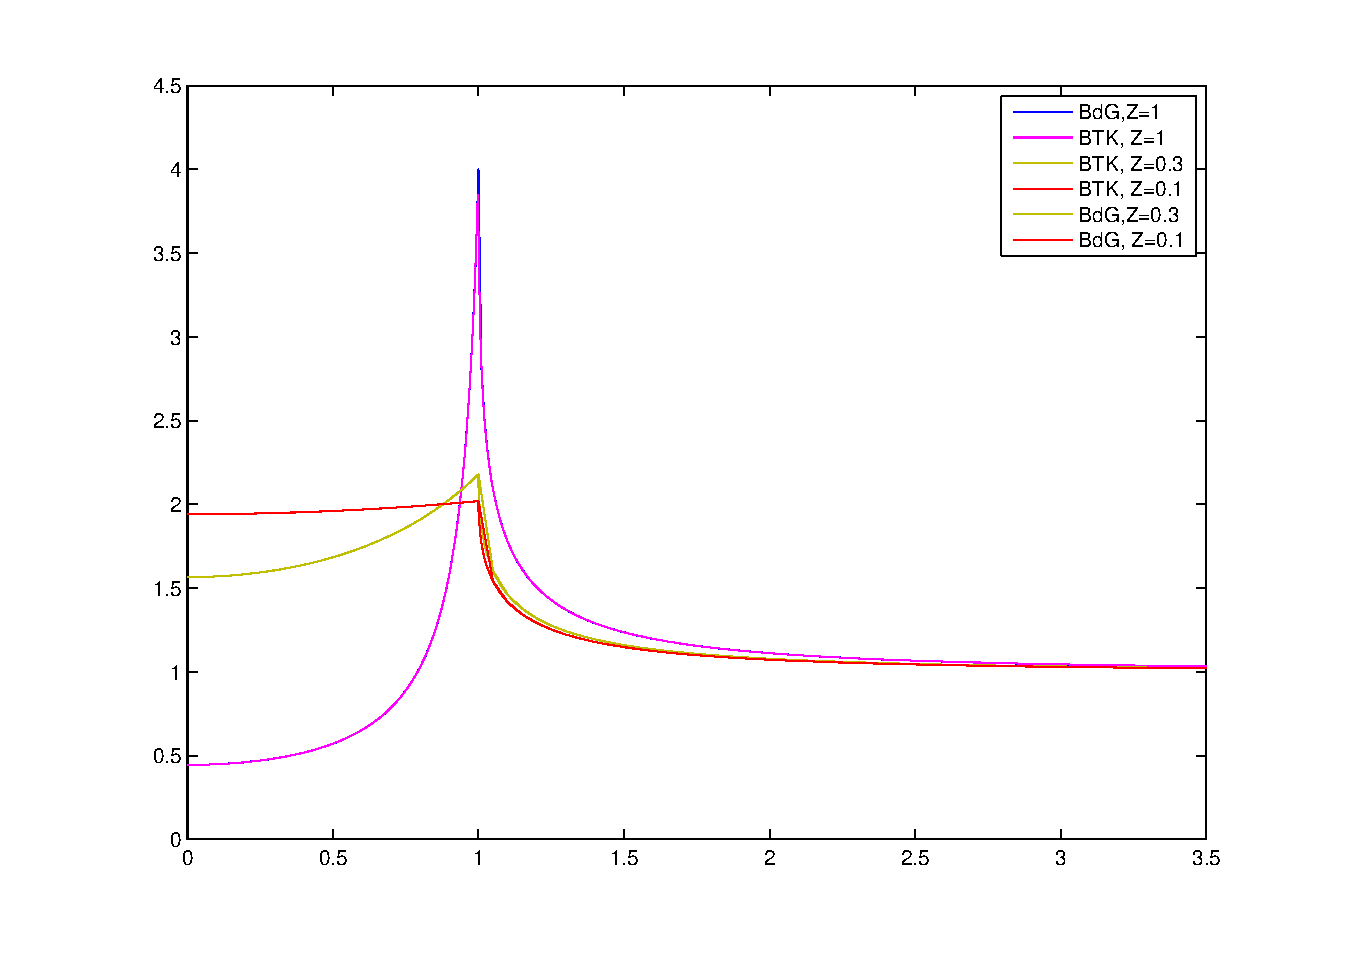
\includegraphics[width=10cm]{./Figures/3-2-8.eps}
		\rule{35em}{0.5pt}
	\caption[An Electron]{BTK case when we set $\Delta_R=1,\Delta_I=0$}
	\label{fig:BTK reproduction}
\end{figure}

Also, when barrier height $Z_0=0$, we should observe flat region with the value of $2$ in the middle, Fig.\ref{fig:z reproduction}.
\begin{figure}[htbp]
\small
	\centering
		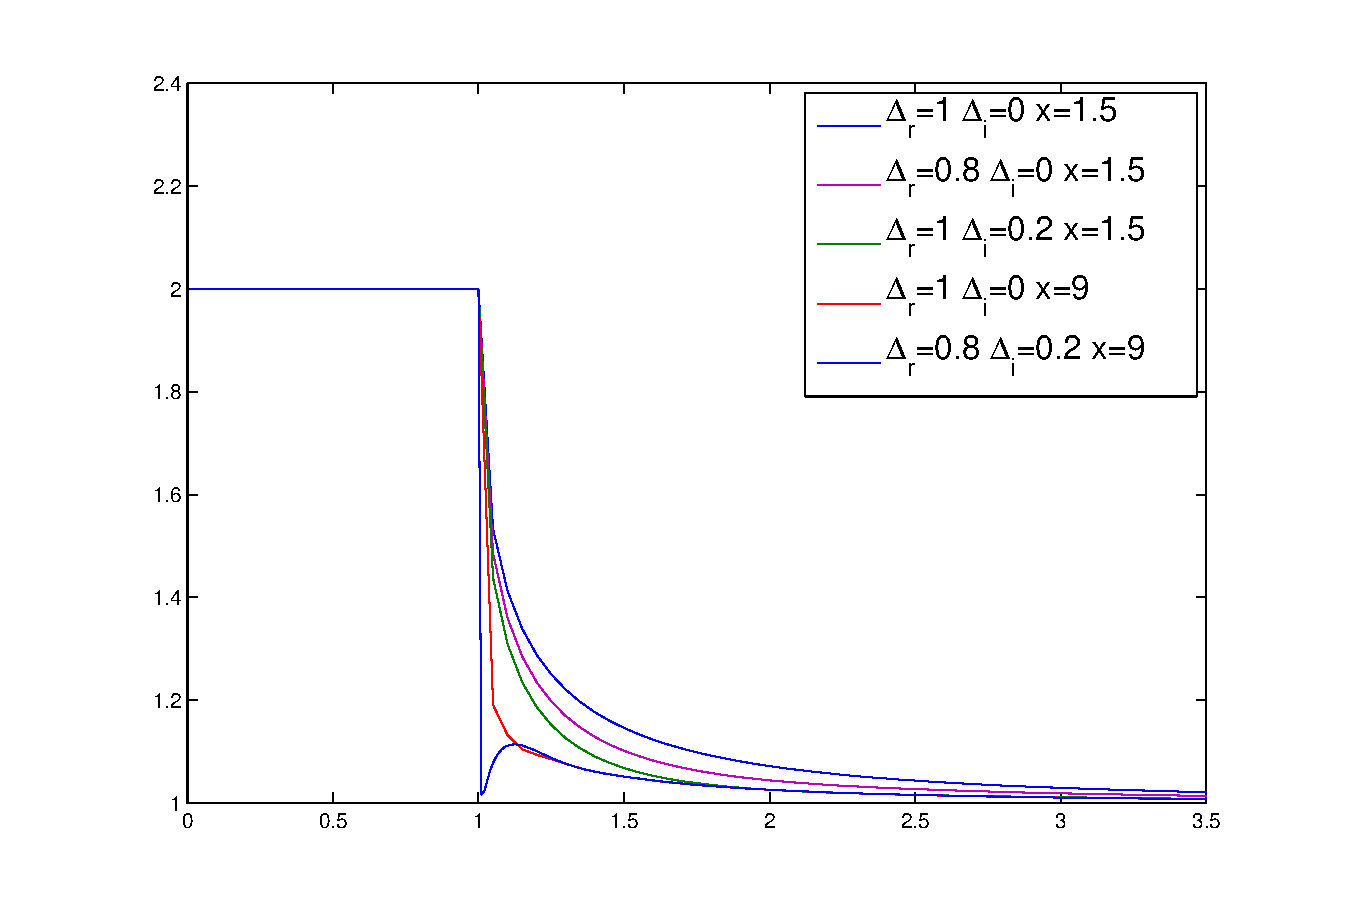
\includegraphics[width=10cm]{./Figures/3-2-9.eps}
		\rule{35em}{0.5pt}
	\caption[An Electron]{The flat region in the middle appears no matter what reduced gap and induced gap and the proximity region thickness are}
	\label{fig:z reproduction}
\end{figure}

\subsection{$s$-wave Proximity Effect at Normal Incident with Various Parameters}
Similar to the procedure in the previous chapter, with solutions obtained, we first have a look at the kernel of the conductance,$\sigma_S$, in \eqref{sub-kernel}.

We draw a list of figures showing the change of the shape according to the varying reduced gap and induced gap, setting the coherence length as $\pi\xi_0=1$, Fig.\ref{Z=0.3reducedthin}-Fig.\ref{Z=0.3induced}.
\begin{figure}[htbp]
\small
\centering
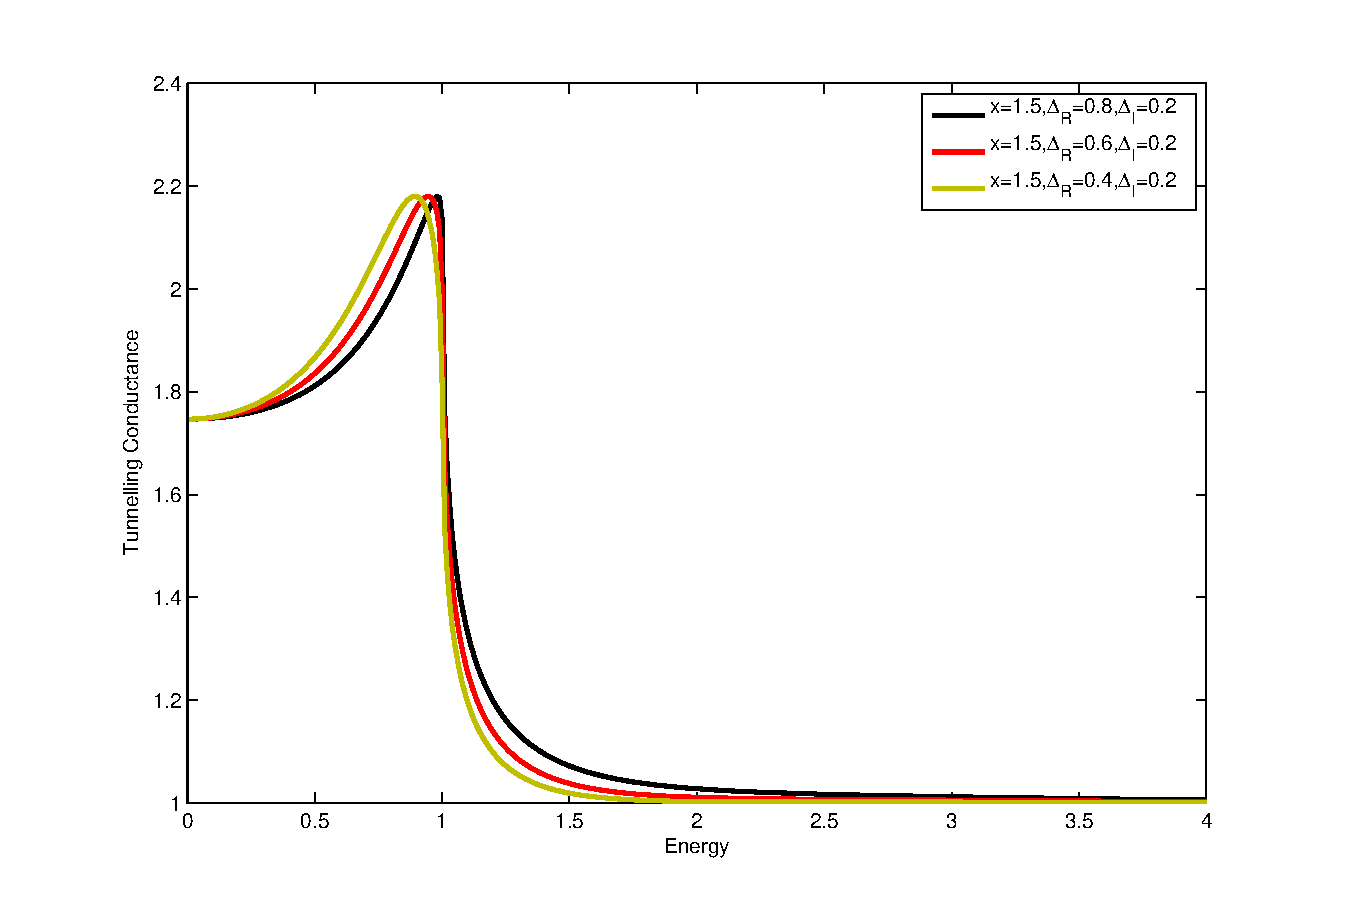
\includegraphics[width=10cm]{3-3-4.eps}
\caption{Low barrier height $Z_0=0.3$ for various values of the reduced gap. We don't see many peaks when the proximity region is thin.}
\label{Z=0.3reducedthin}
\end{figure} 
\begin{figure}[htbp]
\small
\centering
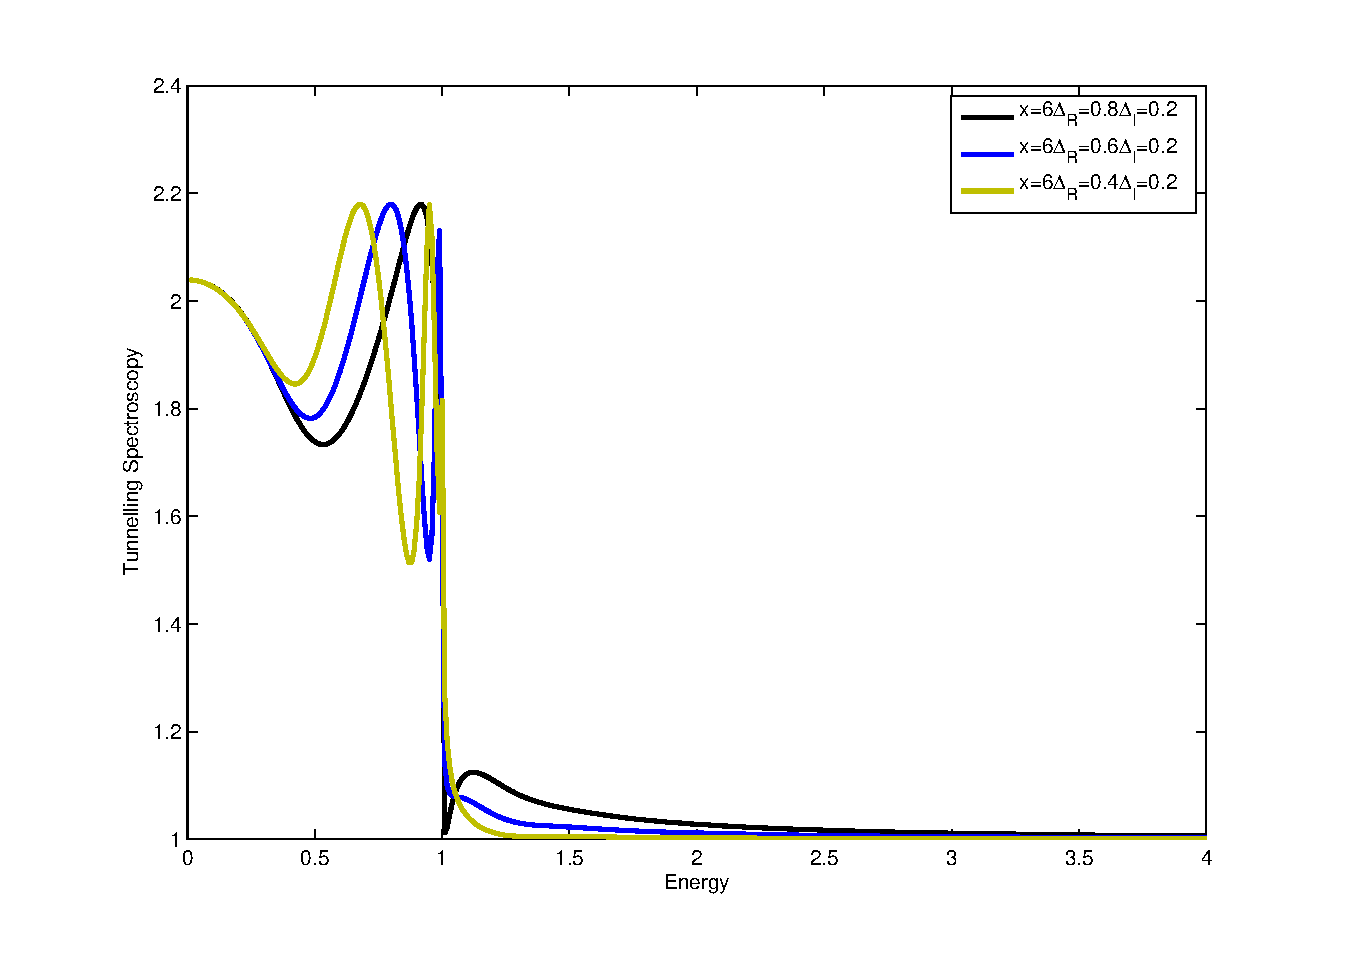
\includegraphics[width=10cm]{3-3-5.eps}
\caption{Some peaks show if thicker proximity region is chosen at low barrier height, with reduced gap varying and included gap fixed.$Z_0=0.3$.}
\label{Z=0.3reduced}
\end{figure}
\begin{figure}[htbp]
\small
\centering
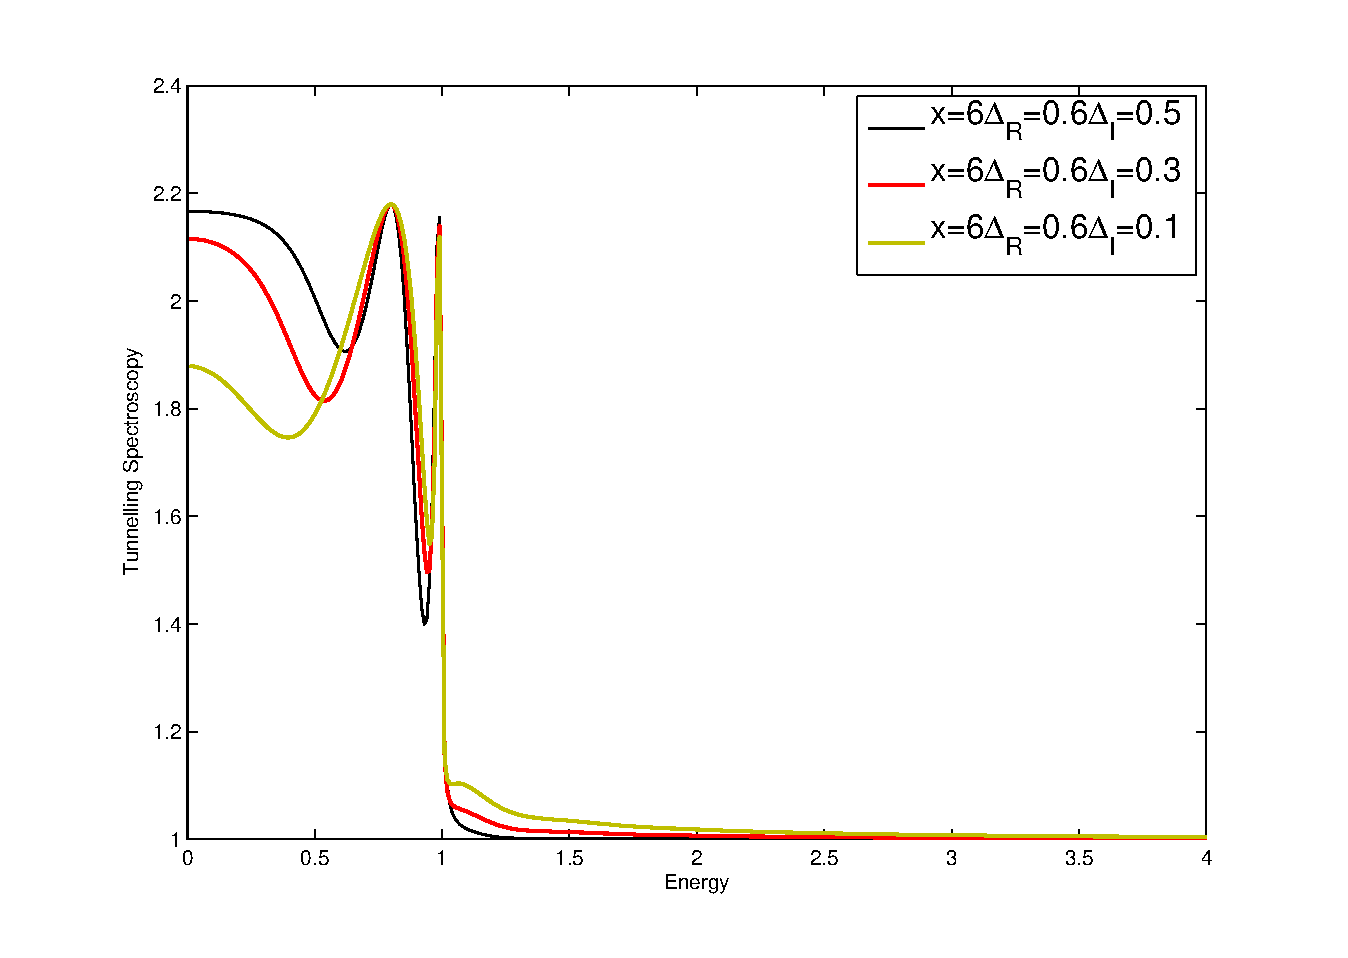
\includegraphics[width=10cm]{3-3-6.eps}
\caption{Some peaks show if thicker proximity region is chosen at low barrier height, with induced gap varying and reduced gap fixed.$Z_0=0.3$.}
\label{Z=0.3induced}
\end{figure}


\begin{comment}
\begin{figure}[htbp]
\small
\centering
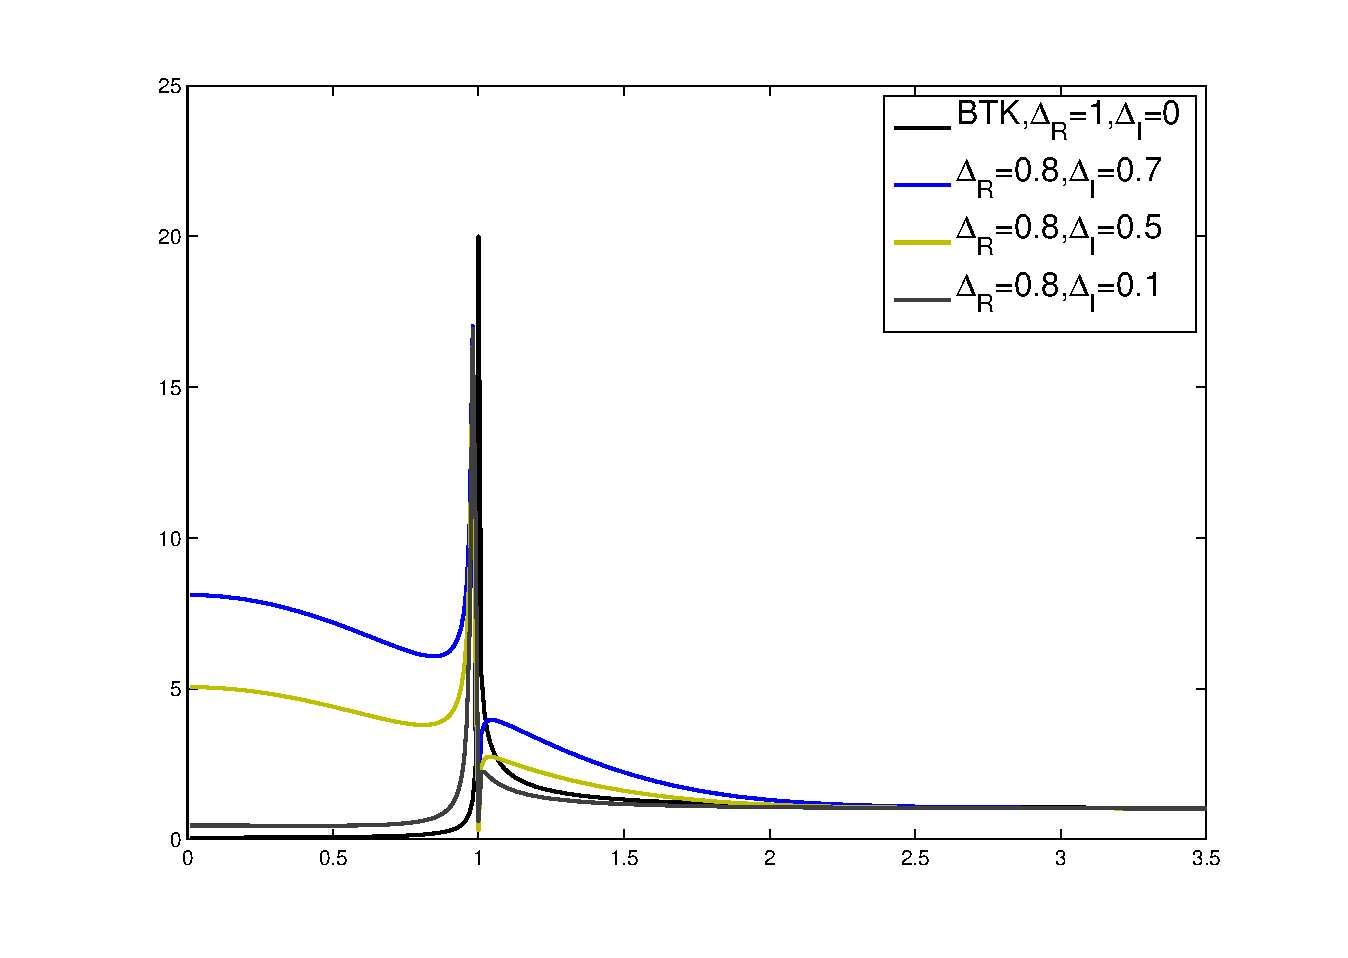
\includegraphics[width=10cm]{3-3-1.eps}
\caption{The figure indicates the difference with induced gap varying.$Z_0=0.3$.}
\label{Z=0.3induced}
\end{figure}
\begin{figure}[htbp]
\small
\centering
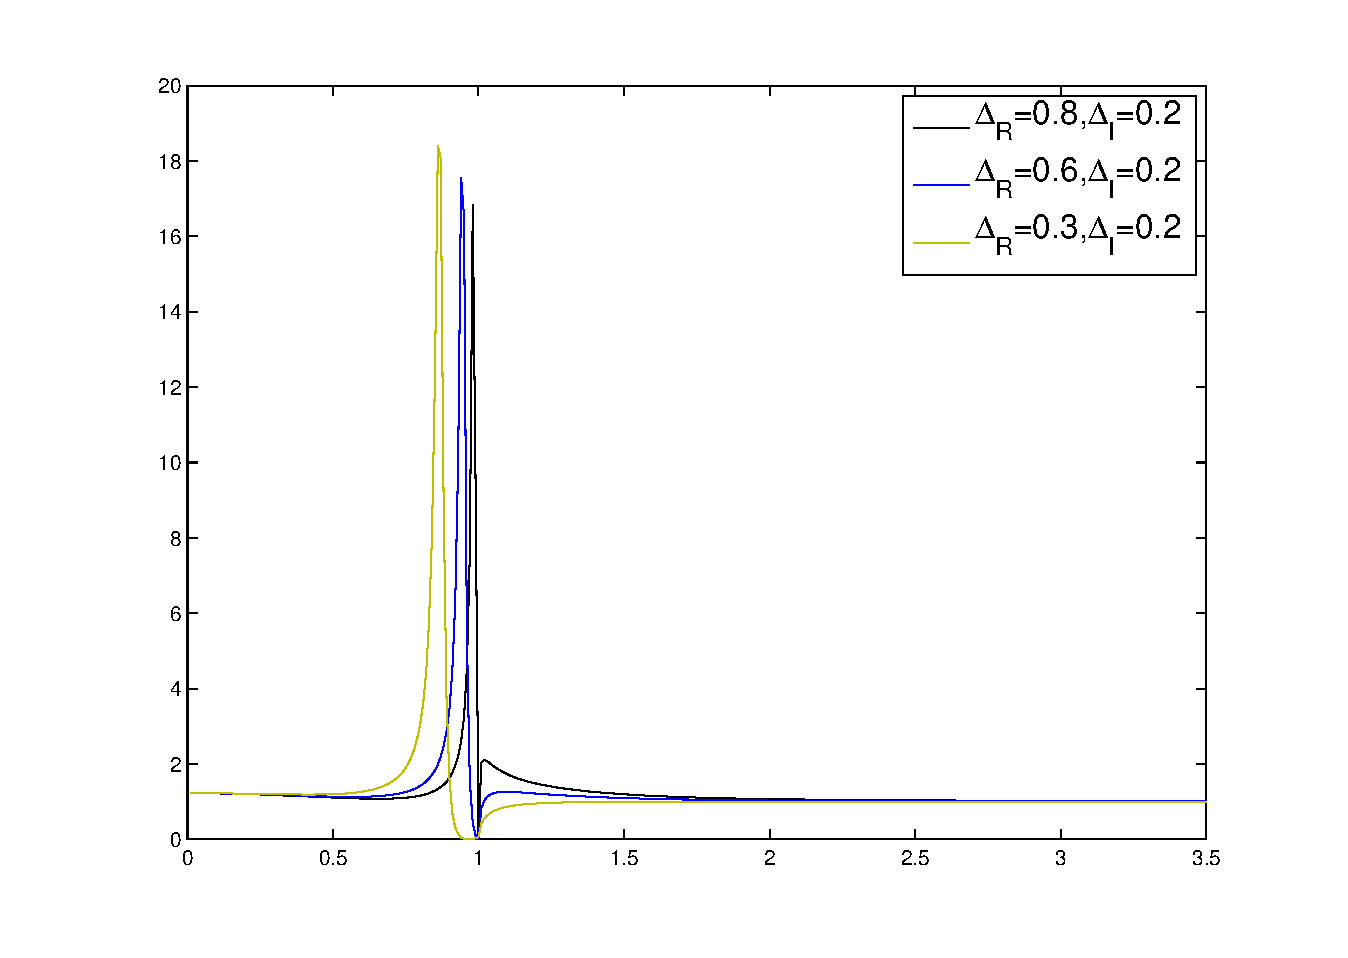
\includegraphics[width=10cm]{3-3-2.eps}
\caption{The figure indicates the difference with reduced gap varying.$Z_0=3$.}
\label{fig:6}
\end{figure}
\end{comment}

Also, as a thought, the proximity region width scaled on the coherence length may affect the transmission. Comparing the plots in Fig.\ref{fig:kernel x} or comparing Fig.\ref{Z=0.3reducedthin} with Fig.\ref{Z=0.3reduced}, we can discover the difference. The thicker proximity region leads to the higher conductance value close to $E=0$ and create more peaks.
\begin{figure}[htbp]
\small
\centering
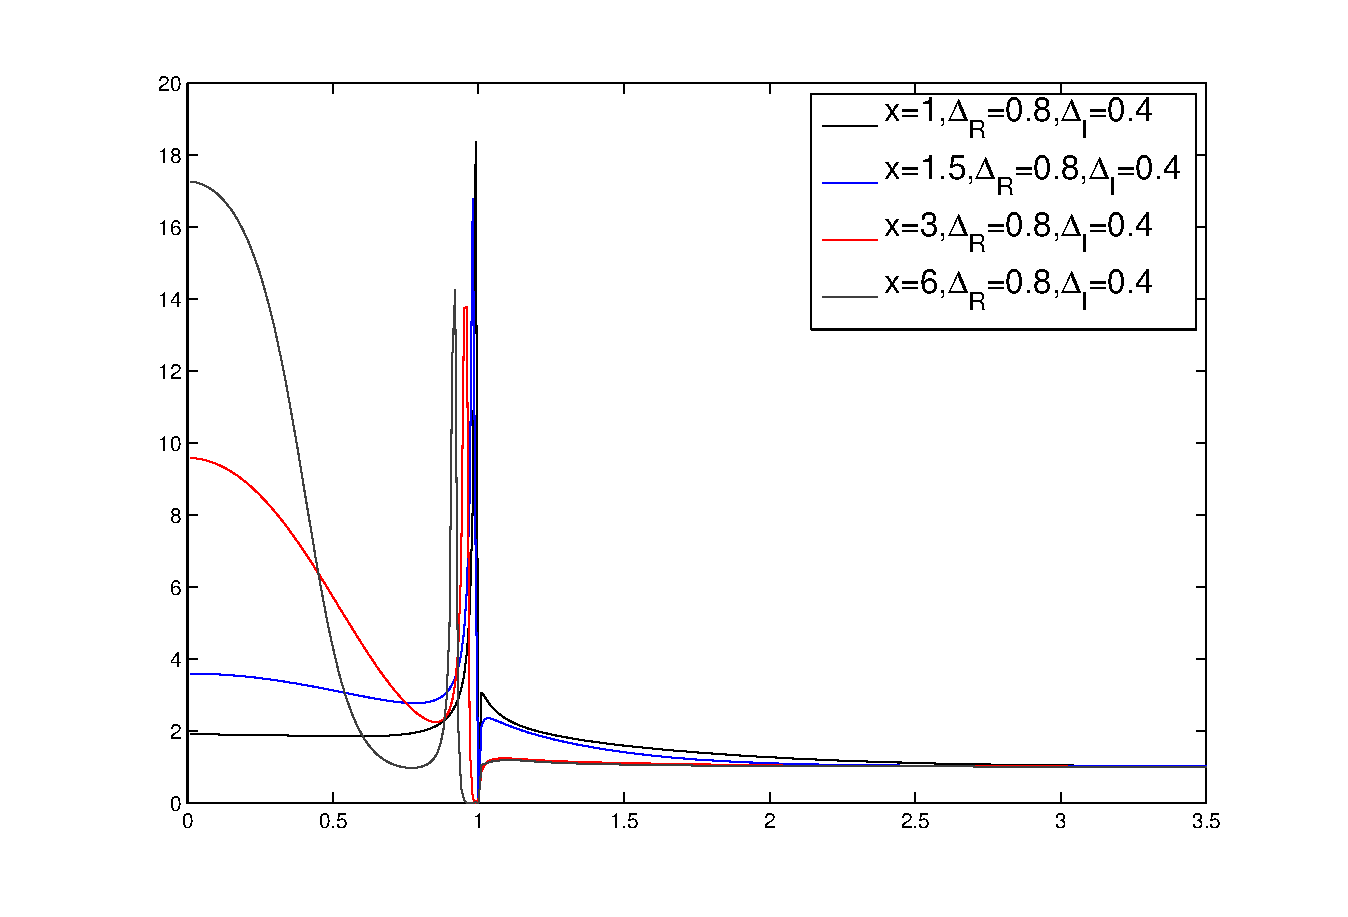
\includegraphics[width=10cm]{3-3-3.eps}
\caption{Increasing the proximity thickness leads to increasing value in the middle and create more peaks. $Z_0=3$}
\label{fig:kernel x}
\end{figure}

The Fig.\ref{MapInduced} and Fig.\ref{MapReduced} gives us a clearer picture of the existence of the reduced gap and induced gap.

In Fig.\ref{MapInduced}, we set bulk gap $\Delta_0=2$, fix the reduced gap $\Delta_r=1$ and vary the induced gap $\Delta_i$ from $0$ to $1.5$.  The red tongue in the middle indicates the properties of the varying induced gap, whose width is from $0$ to about $1.5$, corresponding to the value of induced gap at that point.
\begin{figure}[htbp]
\small
	\centering
		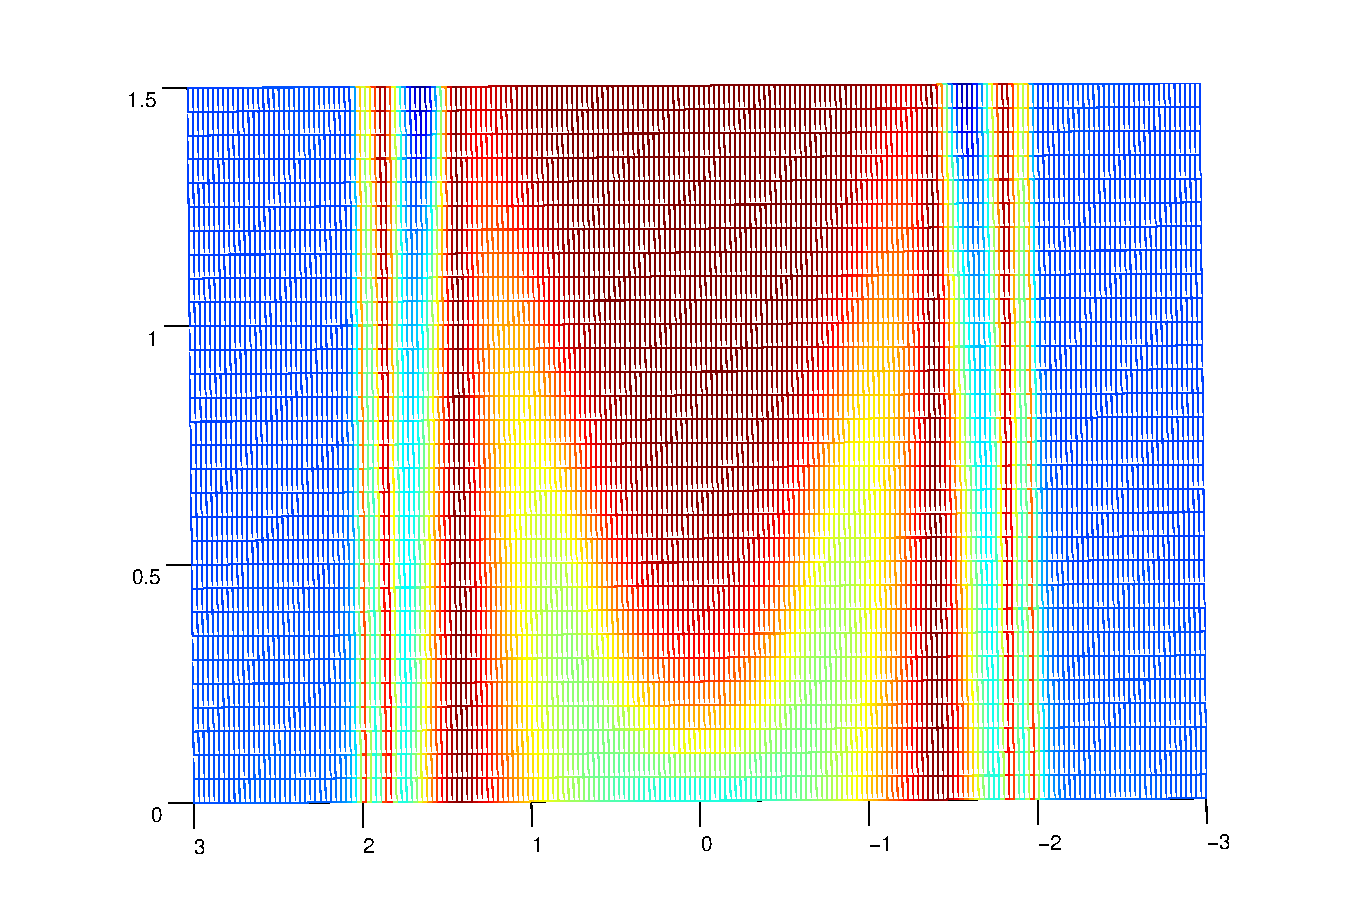
\includegraphics[width=10cm]{./Figures/3dinduce.eps}
		\rule{35em}{0.5pt}
	\caption[An Electron]{The picture shows the properties of the tunnelling conductance when induced gap is varying while reduced gap is fixed. The blue colour indicates the low conductance value while in contrast the red colour indicates the high conductance value.}
	\label{MapInduced}
\end{figure}

In Fig.\ref{MapReduced}, we set bulk gap $\Delta_0=2$, fix the induced gap $\Delta_i=0.4$ and vary the reduced gap $\Delta_r$ from $0$ to $2$.  The red rectangular with $width=0.8$ shows the existence of the induced gap. The two branches growing from the bottom indicates the existence of the reduced gap. The minimum value of the reduced gap in the bottom seems to be expelled by the induced gap that it could not reach $0$ as it should be. The maximum value of the reduced gap is at $1$ as it should be.
\begin{figure}[htbp]
\small
	\centering
		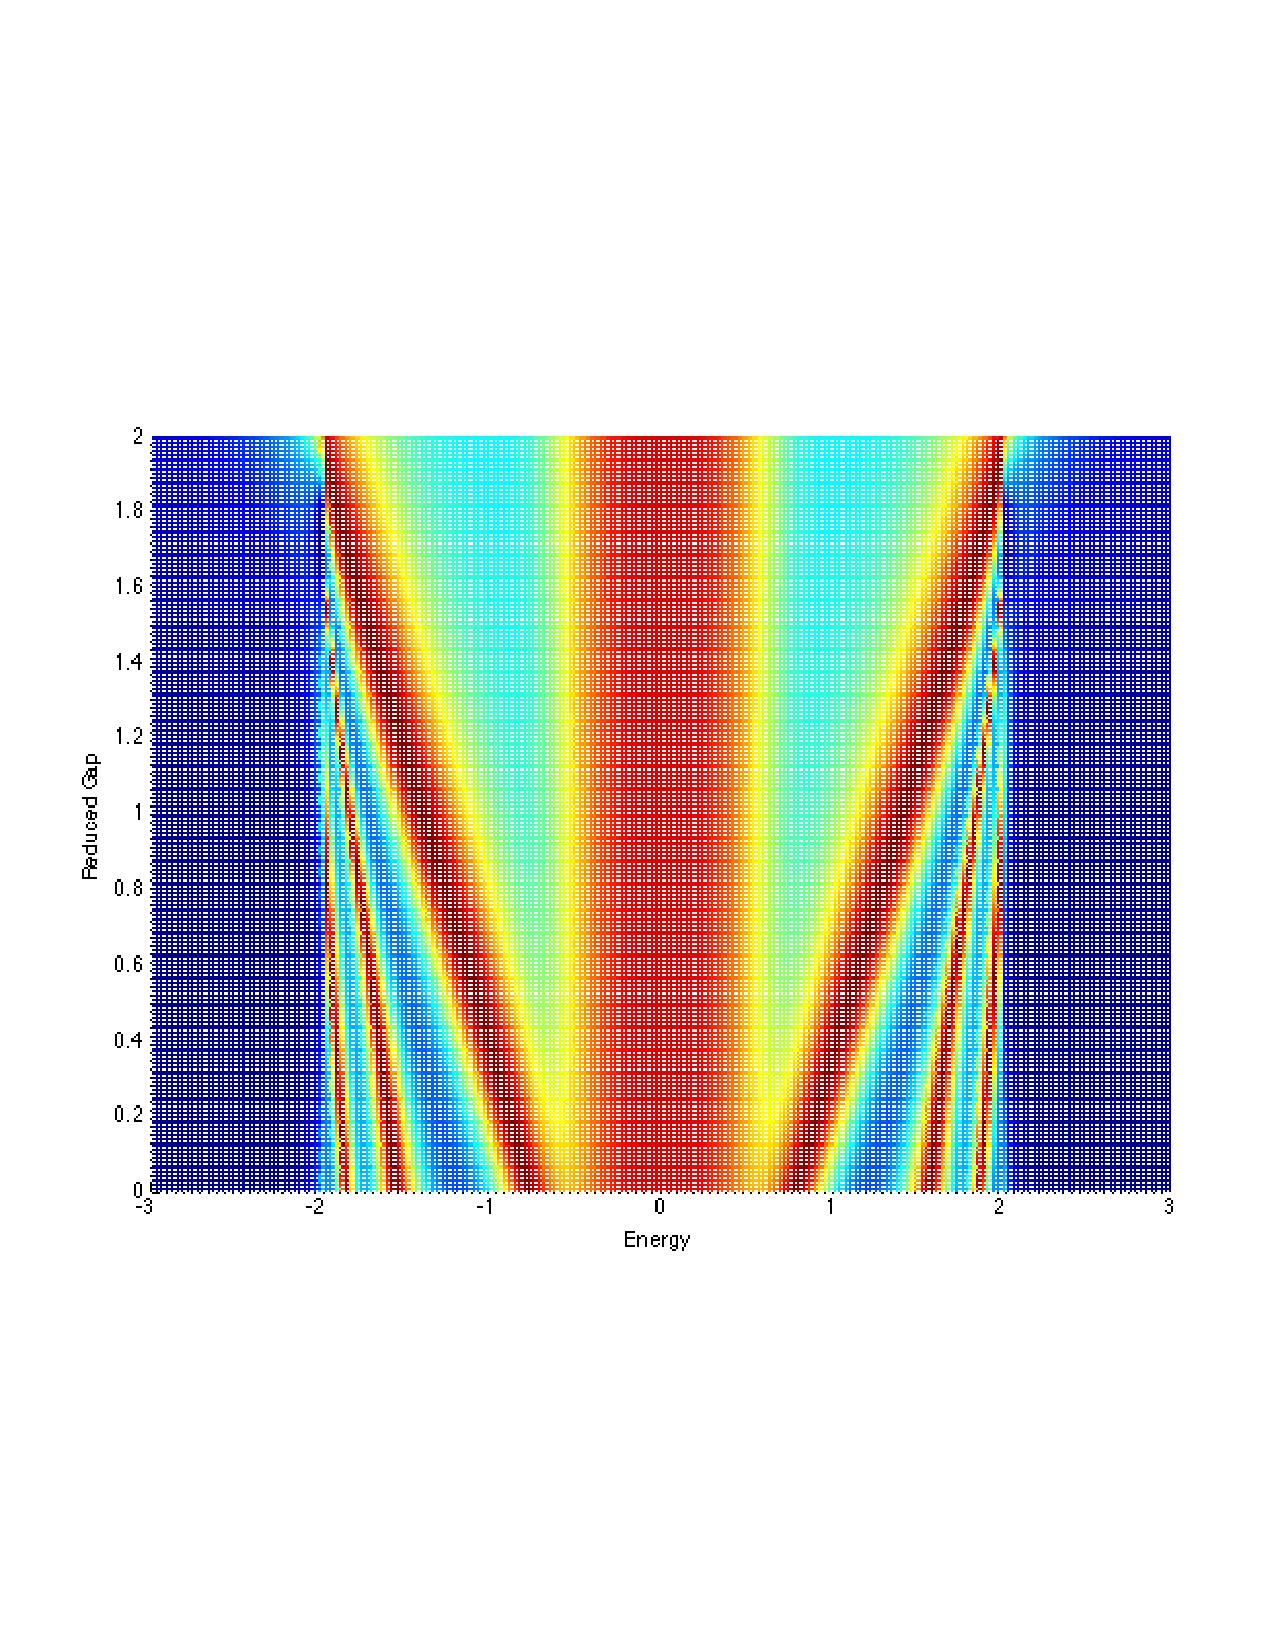
\includegraphics[width=12cm]{./Figures/3dreduceinduce.pdf}
		\rule{35em}{0.5pt}
	\caption[An Electron]{The picture shows the properties of the tunnelling conductance when the reduced gap is varying while the induced gap is fixed. The blue colour indicates the low conductance value while in contrast the red colour indicates the high conductance value.}
	\label{MapReduced}
\end{figure}
%%%%new section
\section{An In Progress Approach to the $d$-wave Tunnelling Spectroscopy with Proximity Effect}
\begin{figure}[htbp]
\small
	\centering
		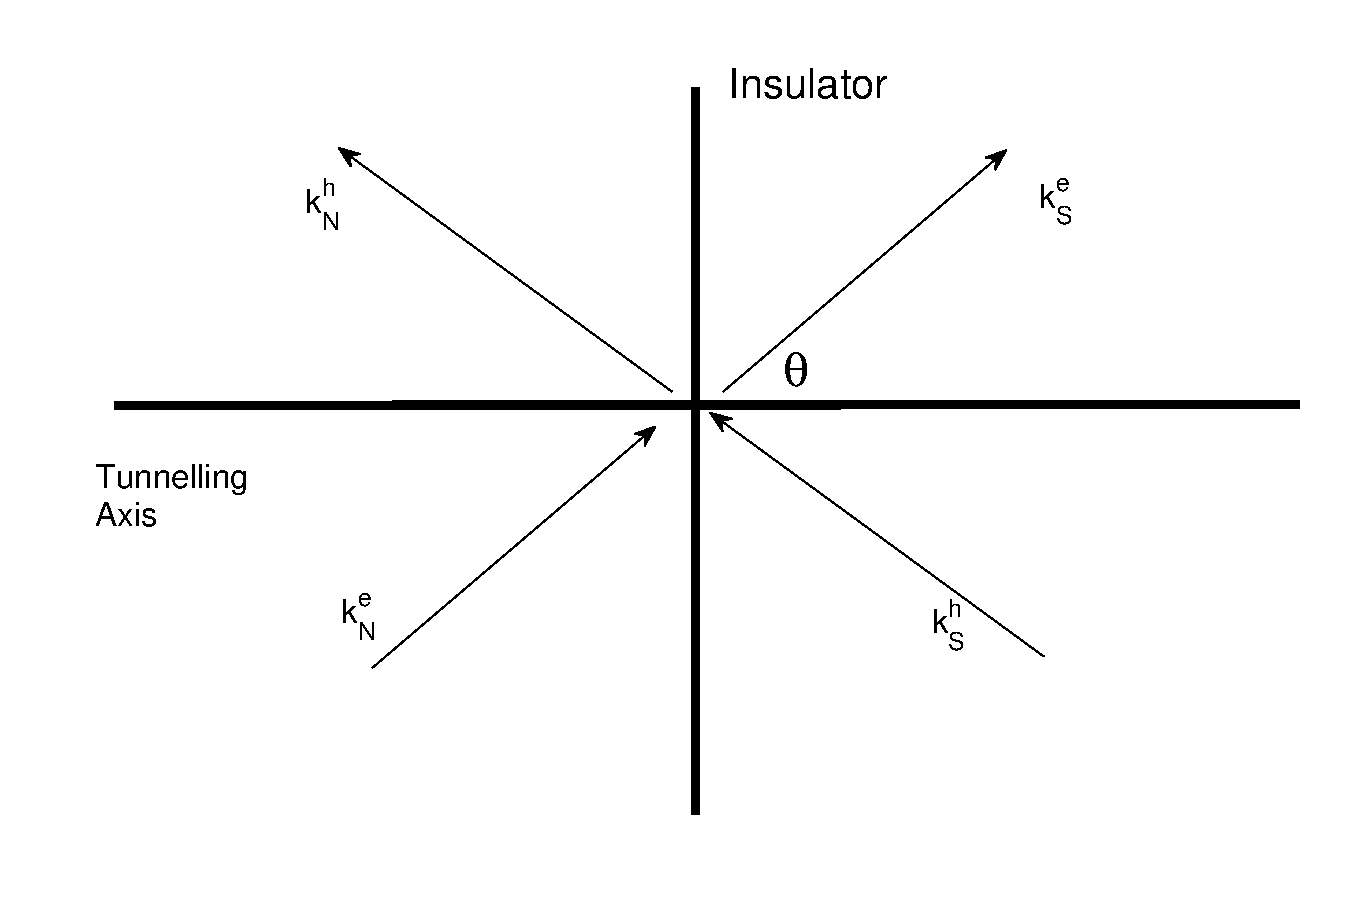
\includegraphics[width=10cm]{./Figures/3-5-1.eps}
		\rule{35em}{0.5pt}
	\caption[An Electron]{The four processes happen at the insulator. $k_S^e$ is the ordinary electron reflection vector;  $k_S^h$ is the hole reflection vector; $k_N^e$ is the electron transmission vector; $k_S^h$ is the hole transmission vector.}
	\label{fig:Andreev}
\end{figure}
In the $d$-wave tunnelling case, the transmission and reflection is interpreted in Fig~\ref{fig:Andreev}.  Note that the wave-vector parallel to the interface are always conserved. For the wave-vectors in the incident plane, we assume that 
\begin{eqnarray}
|\mathbf{k}_N^e|=|\mathbf{k}_S^e|
\end{eqnarray}
According to the momentum conservation law for its interface component,
\begin{eqnarray}
|\mathbf{k}_N^e|\sin\theta_N=|\mathbf{k}_S^e|\sin\theta_S
\end{eqnarray}
so that
\begin{eqnarray}
\theta_S=\theta_N=\theta\nonumber\\
\mathbf{k}_N^e=\mathbf{k}_S^e
\end{eqnarray}

We use $\mathbf{k}$ to express the incident and transmission wave-vectors. In $d$-wave case, the Bogoliubov equations are written as \citep{Reference11}.
\begin{eqnarray}\label{d wave BdG}
&&\DF{\partial u}{\partial z}=i(\pi \xi_0\Delta_0\cos\theta)^{-1}[Eu-\Delta(z)v]\nonumber\\
&&\DF{\partial v}{\partial z}=-i(\pi \xi_0\Delta_0\cos\theta)^{-1}[Ev-\Delta(z)u]\nonumber\\
&&\mathbf{k}\cdot\mathbf{z} = \cos\theta
\end{eqnarray}
And in addition we write another organised Bogoliubov equations for analysis,
\begin{eqnarray}\label{BdG second order}
&&\frac{\partial^2u}{\partial z^2}-\frac{1}{\Delta}\frac{\partial \Delta}{\partial z}\frac{\partial u}{\partial z}+\Big(\frac{i}{B\Delta}\frac{\partial \Delta}{\partial z}E+\frac{E^2-\Delta^2}{B^2}\Big)u=0\nonumber\\
&&\frac{\partial^2v}{\partial z^2}-\frac{1}{\Delta}\frac{\partial \Delta}{\partial z}\frac{\partial v}{\partial z}+\Big(-\frac{i}{B\Delta}\frac{\partial \Delta}{\partial z}E+\frac{E^2-\Delta^2}{B^2}\Big)v=0\\
&&B=\pi\xi_0\Delta_0\cos\theta\nonumber
\end{eqnarray}
After obtaining the $u,v$ values for each incident angle $\theta$ and interface angle $\phi$, we refer to the formulae \eqref{2D-Kernel-Integral} and \eqref{abc}.

Again to make sure the model is correct, we attempt to reproduce $d$-wave BTK here. 
In the case of BTK, we could directly write the terms \eqref{normal condition} as
\begin{eqnarray}\label{BTK normal condition}
&&z_N=z_S=0\nonumber\\
&&u_a=u_0e^{ik_Sz_S},v_a=v_0e^{ik_Sz_S}\nonumber\\
&&u_b=v_0e^{ik_Sz_S},v_b=u_0e^{ik_Sz_S}
\end{eqnarray}
so that the Andreev reflection $a_e$ and the ordinary reflection $b_e$ is can be derived,
\begin{eqnarray}\label{BTK andreev}
|a_e|=\left|\frac{u_0v_0}{(1+Z^2)u_0^2-Z^2v_0^2}\right|\nonumber\\
\\
|b_e|=\left|\frac{iZ(1-iZ)(v_0^2-u_0^2)}{(1+Z^2)u_0^2-Z^2v_0^2}\right|\nonumber
\end{eqnarray}
Note that \eqref{BTK andreev} is identical to \eqref{Tanaka Kernel}, if we set phase difference of the pair potentials as $0$.

We take a look at the $ab$-tunnelling first. Please be aware that in $ab$-tunnelling we DID NOT place the factor $\cos\theta$ in the equation \eqref{d wave BdG} for the specific case of BTK indicated by the reference\citep{Reference2}. This is mathematically derived from the above statements about BTK case, that the factor $\pi\xi_0\Delta_0\cos\theta$ is trivial in the BTK case as the reduced region and induced region don't exist, leading to the fact that the solution is irrelevant to this factor. As indicated in the previous chapter, the pair potential related both to momentum space and position space has the form
\begin{eqnarray}\label{ab momentum position}
\Delta(\theta,z)=|\Delta(z)\cos2\theta|
\end{eqnarray}
where $\Delta(z)$ can be referred to \eqref{spatial form of gap}. Also we choose the absolute value of the pair potential according to the \eqref{BdG second order}. In Fig.\ref{BdGdwaveab}, we could see that the reproduction is fine.
\begin{figure}[htbp]
\small
	\centering
		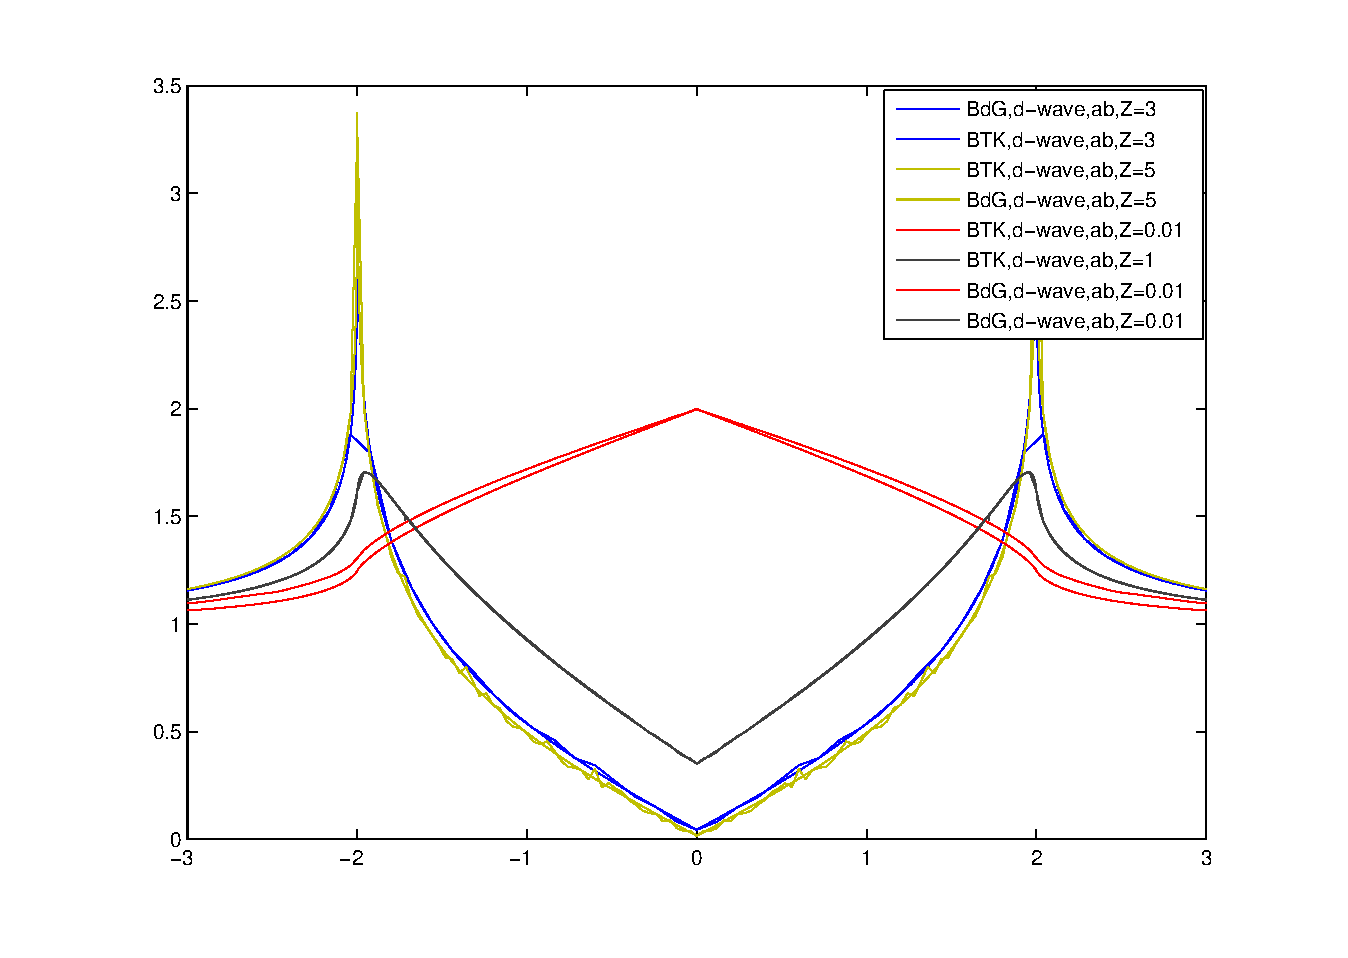
\includegraphics[width=8cm]{./Figures/BdGdwaveab.eps}
		\rule{35em}{0.5pt}
	\caption[An Electron]{The reproduction for the $d_{x^2-y^2}$ $ab$-tunnelling case. $Z_0=0.01,1,3,5$}
	\label{BdGdwaveab}
\end{figure}

In $c$-axis tunnelling in which we are more interested, we set pair potential as
\begin{eqnarray}\label{c momentum position}
\Delta(\varphi,z)=|\Delta(z)\cos2\varphi|
\end{eqnarray}
It can be derived from \eqref{General Energy Gap}. 
\begin{figure}[htbp]
\small
	\centering
		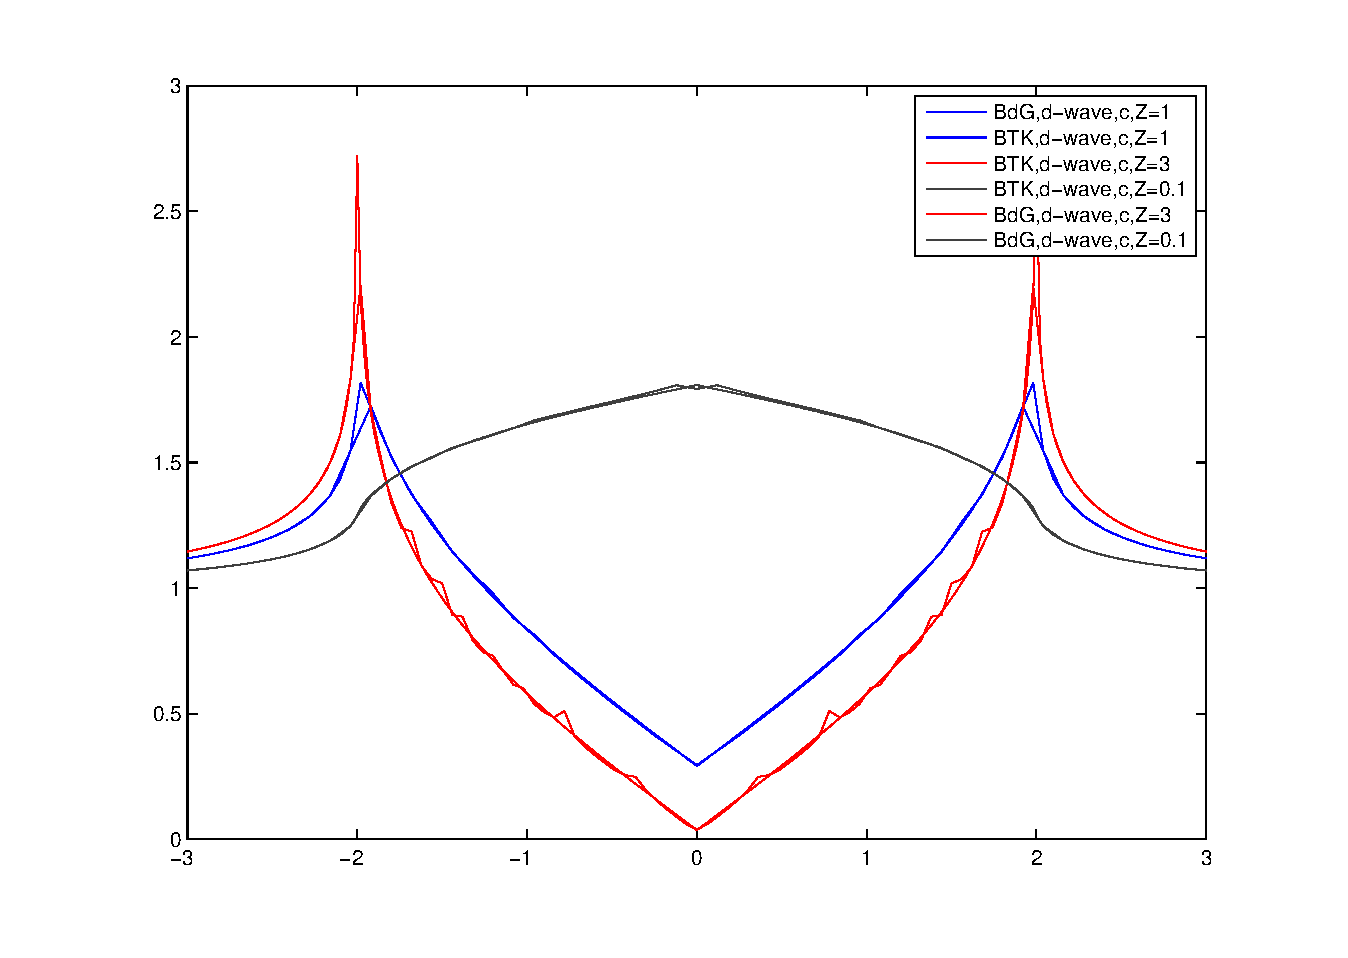
\includegraphics[width=8cm]{./Figures/Dcz.eps}
		\rule{35em}{0.5pt}
	\caption[An Electron]{The reproduction for the $d_{x^2-y^2}$ $c$-tunnelling case. $Z_0=0.1,1,3$}
	\label{Dcz}
\end{figure}
In Fig.\ref{Dcz}, we could see that the reproduction is fine.

We are still working on the $d$-wave proximity tunnelling spectroscopy. We did a trial calculation for the $d$-wave $ab$-tunnelling case. In the calculation, the $\cos\theta$ in \eqref{d wave BdG} is no longer trivial. Also, we can draw the conclusion from \eqref{d wave BdG} that if tunnelling at large incident angle, close to $\pm\pi/2$, the functions $u(z),v(z)$ will oscillate heavily. Meanwhile, $\cos\theta$ in the integral formula \eqref{2D-Kernel-Integral} is relatively small, in the light of which we do not have to do a complete half sphere integration, but within the domain $\theta\in[-1.5,1.5]$, so that a faster computation might be performed.
Fig.\ref{dabfull2-1-0.4} shows the proximity tunnelling conductance, the induced gap is clearly identified by the bulk in the centre. And the reduced gap is indicated by the second peak whose value, however is slightly larger than the reduced gap value. Also, as the figure is plotted in low resolution, we see some unwanted peaks around the bulk gap. Or it might be caused by the resonance due to thick proximity domain.  Fig.\ref{dabfullfull} shows the proximity tunnelling conductance with various reduced gaps and induced gaps. We can observe that with the same induced gap, the plots share the same bulk in the middle, similar to the figures of normal incident kernel Fig.\ref{Z=0.3reducedthin}-Fig.\ref{Z=0.3induced}. Fig.\ref{dabfullfull} shows additional plots for comparison.
\begin{figure}[htbp]
\small
	\centering
		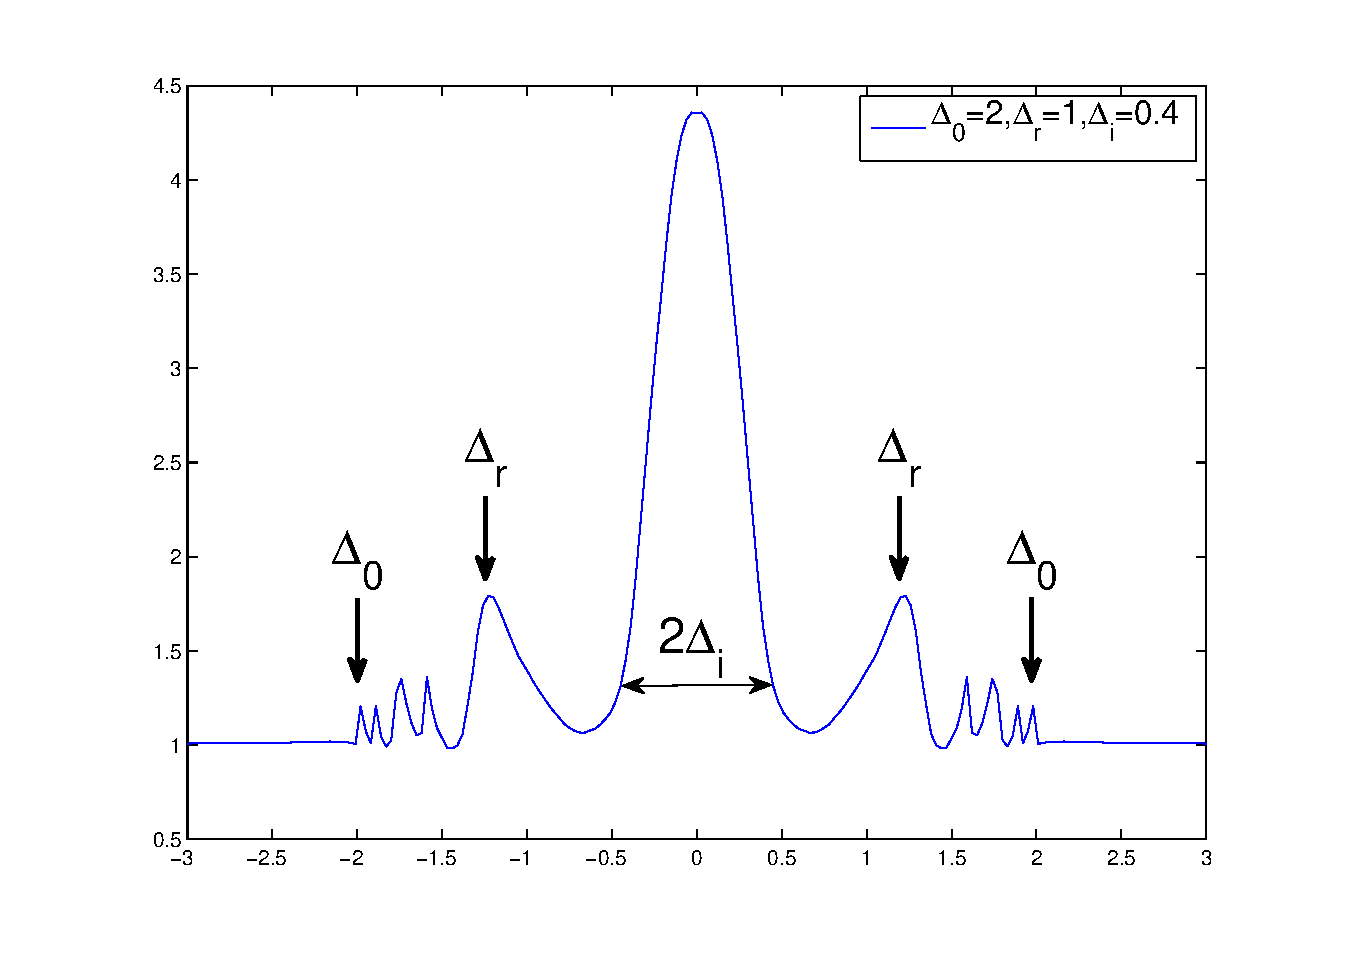
\includegraphics[width=8cm]{./Figures/fulldab2104.eps}
		\rule{35em}{0.5pt}
	\caption[An Electron]{The tunnelling conductance with bulk gap $\Delta_0=2$, reduced gap $\Delta_r=1$, $\Delta_i=0.4$, which are indicated in the figure. We can see that at the bulk gap side there are some oscillations, which may be due to the resolution of the calculation. $Z_0=1$}
	\label{dabfull2-1-0.4}
\end{figure}
\begin{figure}[htbp]
\small
	\centering
		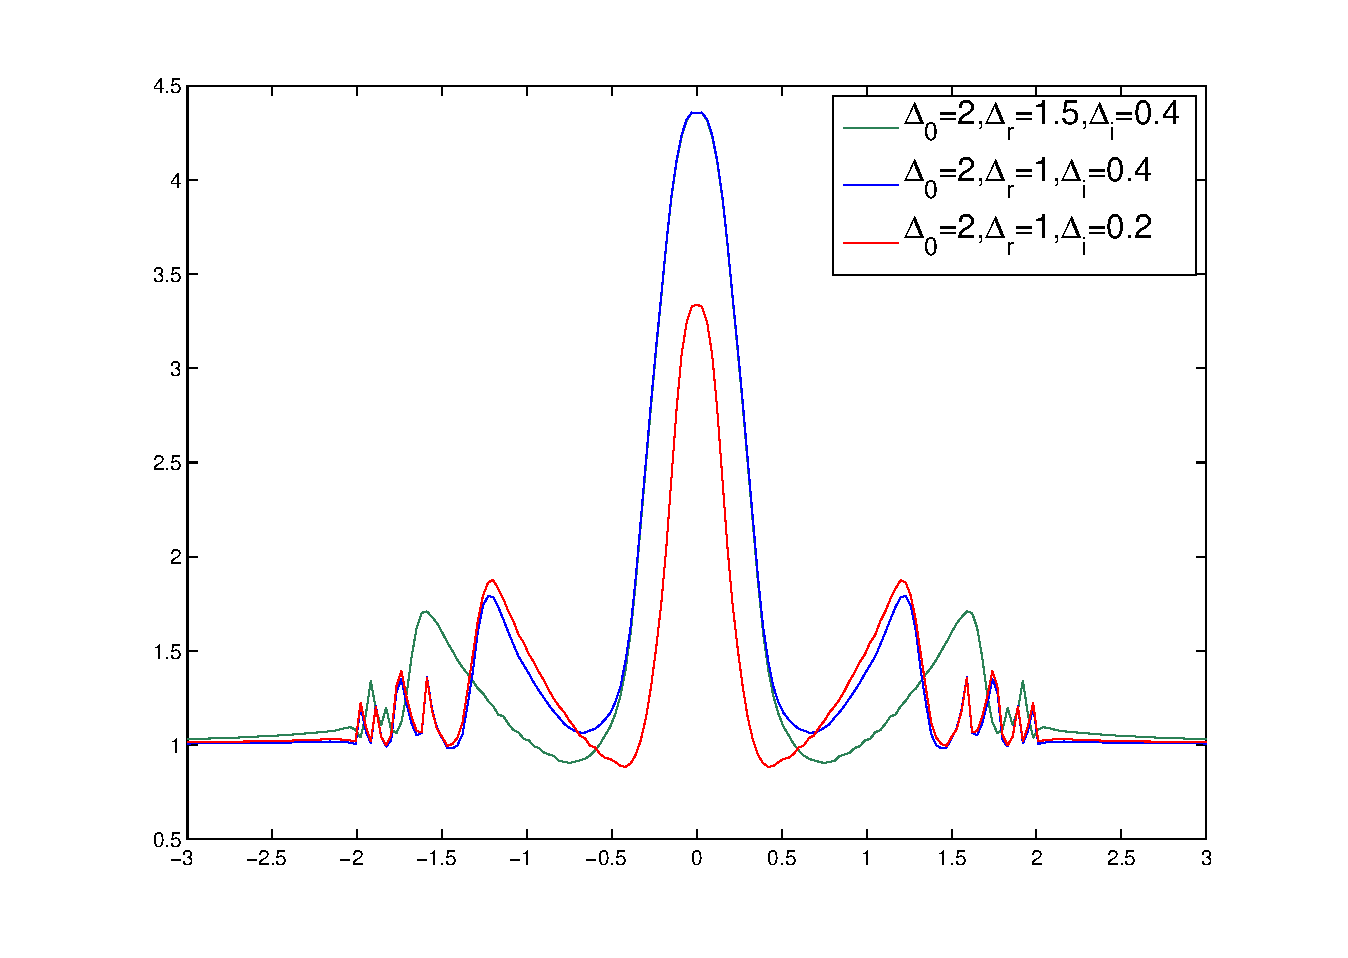
\includegraphics[width=8cm]{./Figures/fulldabfull.eps}
		\rule{35em}{0.5pt}
	\caption[An Electron]{The tunnelling conductance with various reduced gaps and induced gaps. $Z_0=1$.}
	\label{dabfullfull}
\end{figure}

Now we approach the $d$-wave $c$-tunnelling conductance. Similar to the case of $ab$-tunnelling, we conduct the integration within the domain $\varphi\in[0,2\pi], \theta\in[0,1.5]$. Fig.\ref{dcnewsingle} shows the proximity tunnelling conductance, the induced gap is clearly identified by the bulk in the centre. And the reduced gap is indicated by the second peak whose value, however is slightly larger than the reduced gap value. The shape of $c$-tunnelling conductance is quite similar to that of $ab$-tunnelling. Fig.\ref{dcnewfull} shows additional plots for comparison.
\begin{figure}[htbp]
\small
	\centering
		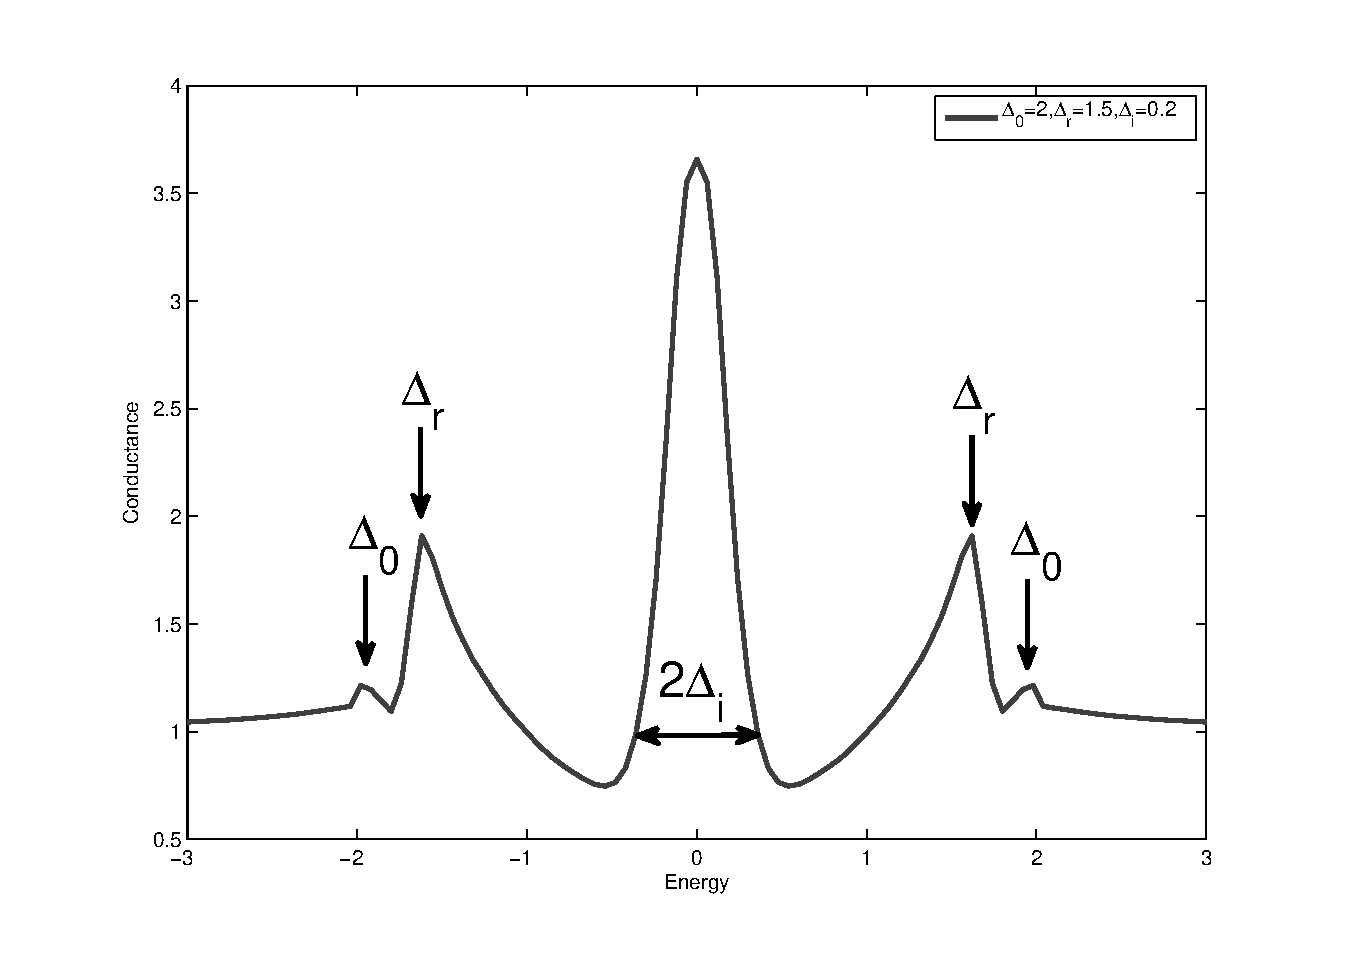
\includegraphics[width=8cm]{./Figures/dcnewsingle.eps}
		\rule{35em}{0.5pt}
	\caption[An Electron]{The tunnelling conductance with bulk gap $\Delta_0=2$, reduced gap $\Delta_r=1.5$, $\Delta_i=0.2$, which are indicated in the figure. $Z_0=1$}
	\label{dcnewsingle}
\end{figure}
\begin{figure}[htbp]
\small
	\centering
		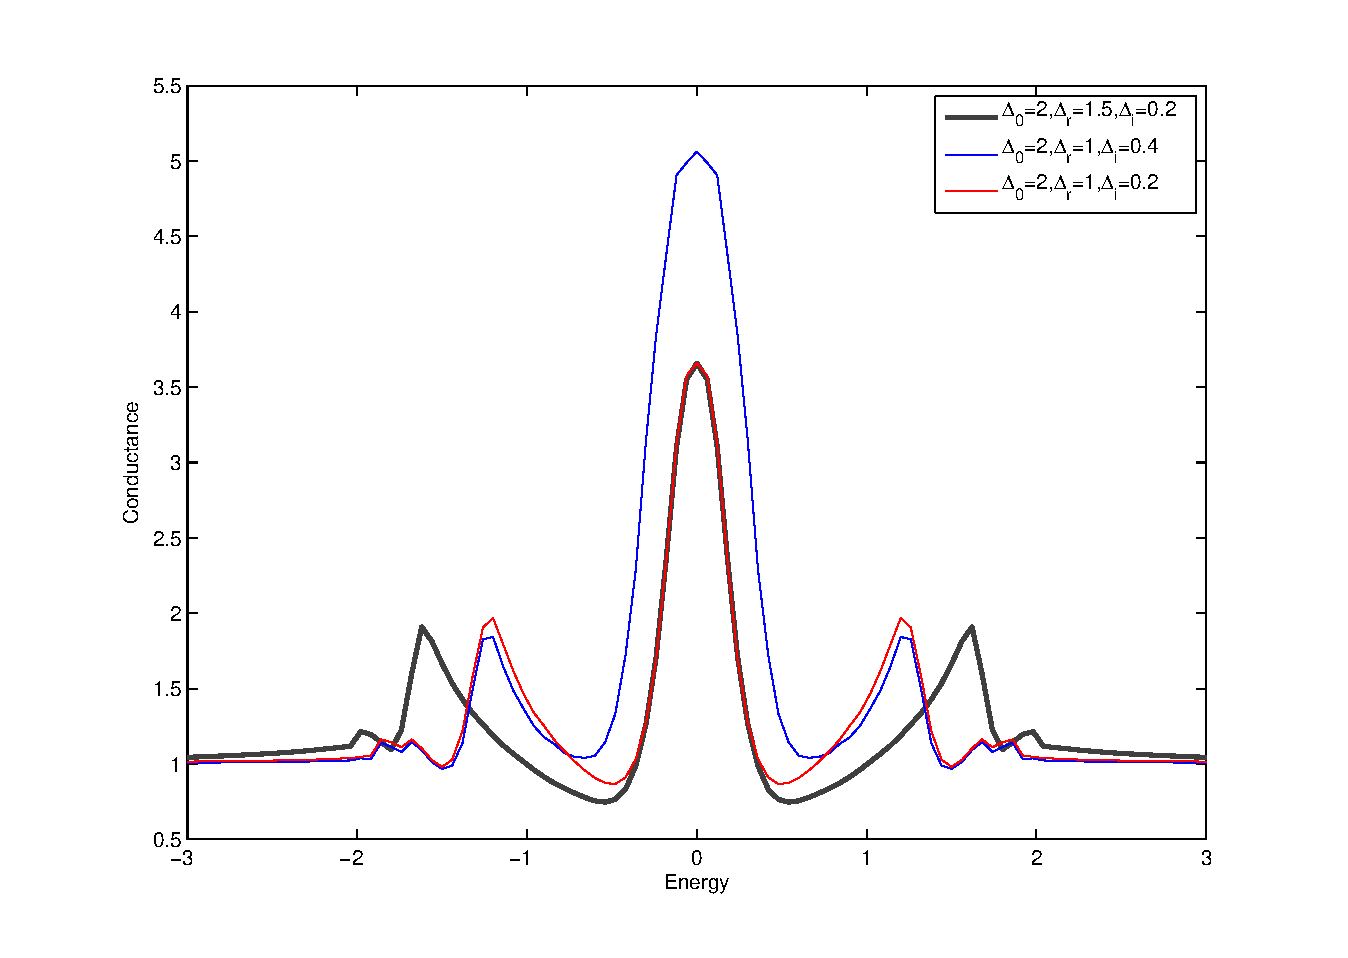
\includegraphics[width=8cm]{./Figures/dcnewfull.eps}
		\rule{35em}{0.5pt}
	\caption[An Electron]{The tunnelling conductance with various reduced gaps and induced gaps. $Z_0=1$.}
	\label{dcnewfull}
\end{figure}

























 % Experimental Setup

% Chapter 1

\chapter{Future Work} % Write in your own chapter title
\label{Chapter4}
\lhead{Chapter 4. \emph{Future Work}} % Write in your own chapter title to set the page header
We conclude our work of calculating $d$-wave tunnelling spectroscopy and fitting the experimental data as well as the calculation the tunnelling spectroscopy accounting for proximity effect.

For the work described in Chapter 2, first of all we need to modify our model. As stated at the end of Chapter 2, the density of states is assumed to be constant, which might probably not be true. Also, we need to perform a calculation using genetic algorithm which is more reliable.

For the work calculating the proximity effect, though it reproduces quite well for the special cases, the picture of reduced gap and induced gap is blurred; we do not have a clear idea of what their effects are. Moreover, we need to have a deeper study of the $d$-wave tunnelling spectroscopy with proximity effect.

 % Experiment 1

% Chapter 1

\chapter{Additional Projects} % Write in your own chapter title
\label{Chapter5}
\lhead{Chapter 5. \emph{Additional Projects}} % Write in your own chapter title to set the page header


\section{Control System for Raman Stage and Fresnel Rhomb} 
The software I designed integrates the XYZ stage control panel and the Fresnel Rhomb control panel. Users can operate XYZ stage and the Fresnel Rhomb at the same time with convenience.
    For XYZ stage control part, apart from controlling the stage, users can store the positions of their samples that may be studied later.
    For Fresnel control part, the digits shown on the software are really polarization angles so that users do not need to convert the units. In addition, a polarization clock is provided to assist the operation. What is more, the COM interface is also adjustable even in the case that the software is installed in a substituted computer.

\begin{figure}[htbp]
         \small
	\centering
		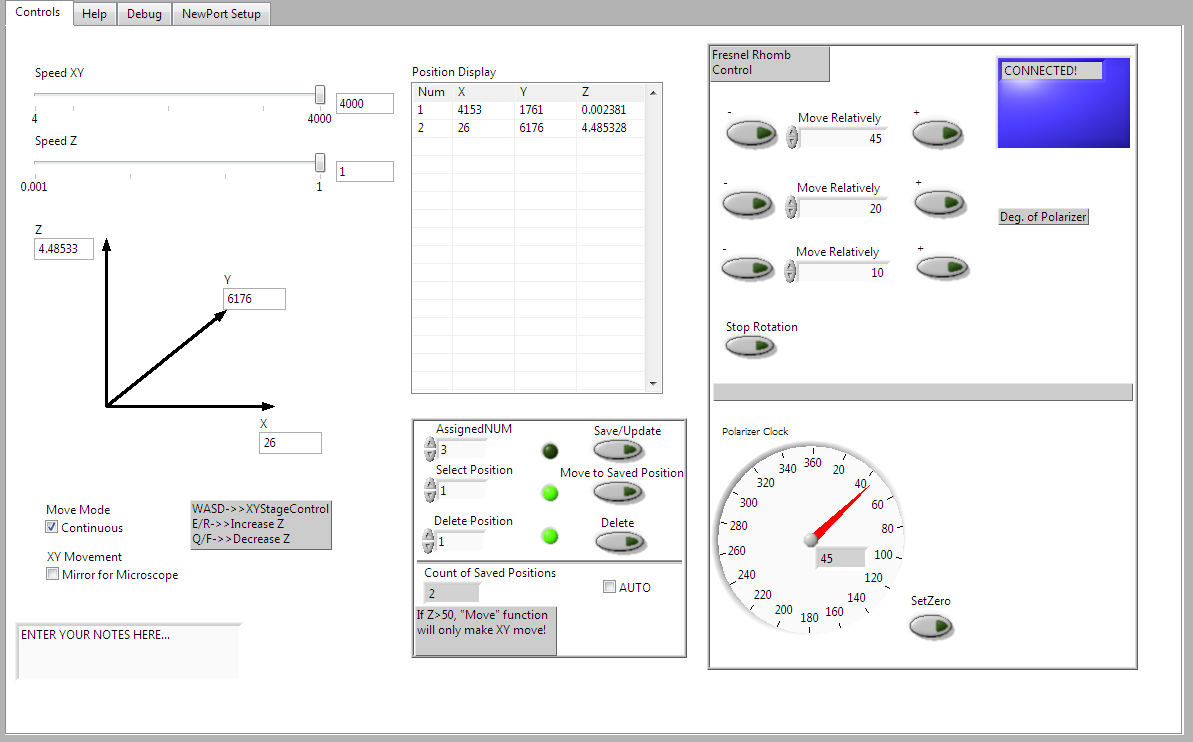
\includegraphics[width=13cm]{./Figures/panel.png}
		\rule{35em}{0.5pt}
	\caption[An Electron]{Main Control Panel}
	\label{fig:Electron}
\end{figure}
 % Experiment 2

%\input{./Chapters/Chapter6} % Results and Discussion

%\input{./Chapters/Chapter7} % Conclusion

%% ----------------------------------------------------------------
% Now begin the Appendices, including them as separate files

\addtocontents{toc}{\vspace{2em}} % Add a gap in the Contents, for aesthetics

%\appendix % Cue to tell LaTeX that the following 'chapters' are Appendices

%% Appendix A

\chapter{Appendix Title Here}
\label{AppendixA}
\lhead{Appendix A. \emph{Appendix Title Here}}

Write your Appendix content here.	% Appendix Title

%\input{./Appendices/AppendixB} % Appendix Title

%\input{./Appendices/AppendixC} % Appendix Title

%\addtocontents{toc}{\vspace{2em}}  % Add a gap in the Contents, for aesthetics
%\backmatter

%% ----------------------------------------------------------------
\label{Reference}
\lhead{\emph{Reference}}  % Change the left side page header to "Bibliography"
\bibliographystyle{ieeetr}%{unsrtnat}  % Use the "unsrtnat" BibTeX style for formatting the Bibliography
\bibliography{Bibliography}  % The references (bibliography) information are stored in the file named "Bibliography.bib"

\end{document}  % The End
%% ----------------------------------------------------------------